\documentclass[10pt,letterpaper]{article}
\usepackage[top=0.85in,left=2.00in,footskip=0.75in]{geometry}

% Use adjustwidth environment to exceed column width (see example table in text)
\usepackage{changepage}

% Use Unicode characters when possible
\usepackage[utf8]{inputenc}

% textcomp package and marvosym package for additional characters
\usepackage{textcomp,marvosym}

% fixltx2e package for \textsubscript
\usepackage{fixltx2e}

% amsmath and amssymb packages, useful for mathematical formulas and symbols
\usepackage{amsmath,amssymb}

% cite package, to clean up citations in the main text. Do not remove.
\usepackage{cite}

%lstlisting
\usepackage{listings}

% Use nameref to cite supporting information files (see Supporting Information section for more info)
\usepackage{nameref}
%\usepackage{hyperref}

% line numbers
\usepackage[right]{lineno}

% ligatures disabled
\usepackage{microtype}
%\DisableLigatures[f]{encoding = *, family = * }

% rotating package for sideways tables
\usepackage{rotating}

% Remove comment for double spacing
%\usepackage{setspace} 
%\doublespacing
\usepackage[lofdepth,lotdepth]{subfig}
% Text layout
%\raggedright
\setlength{\parindent}{0.5cm}
\textwidth 5.25in 
\textheight 8.75in

% Bold the 'Figure #' in the caption and separate it from the title/caption with a period
% Captions will be left justified
\usepackage[aboveskip=1pt,labelfont=bf,labelsep=period,justification=raggedright,singlelinecheck=off]{caption}

% Use the PLoS provided BiBTeX style
\bibliographystyle{plos2009}

% Remove brackets from numbering in List of References
\makeatletter
\renewcommand{\@biblabel}[1]{\quad#1.}
\makeatother

% Leave date blank
\date{15.03.16}

% Header and Footer with logo
%\usepackage{lastpage,fancyhdr,graphicx}
%\pagestyle{myheadings}
%\pagestyle{fancy}
%\fancyhf{}
%\lhead{\includegraphics[natwidth=1.3in,natheight=0.4in]{PLOSlogo.png}}
%\rfoot{\thepage/\pageref{LastPage}}
%\renewcommand{\footrule}{\hrule height 2pt \vspace{2mm}}
%\fancyheadoffset[L]{2.25in}
%\fancyfootoffset[L]{2.25in}
%\lfoot{\sf PLOS}

%% Include all macros below

%\newcommand{\lorem}{{\bf LOREM}}
%\newcommand{\ipsum}{{\bf IPSUM}}

%% END MACROS SECTION


\begin{document}
\vspace*{0.30in}

% Title must be 150 characters or less
\begin{flushleft}
{\Large
\textbf\newline{\LARGE \textbf{Tecnologie Digitali - Relazione di Laboratorio: Caratteristica I-V di un diodo pn da remoto}}
}
\newline
% Insert Author names, affiliations and corresponding author email.
\\
Salvatore Bottaro\textsuperscript{1,*}
Lorenzo Maria Perrone\textsuperscript{1, $\dagger$},
%Name2 Surname\textsuperscript{2,\textpilcrow},
%Name3 Surname\textsuperscript{2,\textcurrency a},
%Name4 Surname\textsuperscript{2,\ddag},
%Name5 Surname\textsuperscript{2,\ddag},
%Name6 Surname\textsuperscript{2,\Yinyang},
%Name7 Surname\textsuperscript{3,*,\Yinyang}
\\
\bf{1} Dipartimento di Fisica, Università di Pisa
\\
%\bf{2} Affiliation Dept/Program/Center, Institution Name, City, State, Country
%\\
%\bf{3} Affiliation Dept/Program/Center, Institution Name, City, State, Country
%\\

% Insert additional author notes using the symbols described below. Insert symbol callouts after author names as necessary.
% 
% Remove or comment out the author notes below if they aren't used.
%
% Primary Equal Contribution Note
%\Yinyang These authors contributed equally to this work.

% Additional Equal Contribution Note
%\ddag These authors also contributed equally to this work.

% Current address notes
%\textcurrency a Insert current address of first author with an address update
% \textcurrency b Insert current address of second author with an address update
% \textcurrency c Insert current address of third author with an address update

% Deceased author note
%\dag Deceased

% Group/Consortium Author Note
%\textpilcrow Insert Collaborative Author line here

* E-mail: salvo.bottaro@hotmail.it\\
$\dagger$ E-mail: lorenzo.perrone.lmp@gmail.com
\end{flushleft}

\section{Acquisizione dei dati e panoramica della strumentazione}
In questa esperienza, uno degli aspetti che abbiamo approfondito consiste nell'acquisizione dei dati relativi alla caratteristica I-V di un diodo da remoto: la strumentazione, comprendente un termostato per la regolazione della temperatura, una scheda di acquisizione dati che acquisisce le tensioni e le correnti ai capi di un diodo, e ovviamente il diodo stesso, si trovavano infatti dislocati in una stanza a cui non si poteva accedere. La procedura di acquisizione è stata dunque completamente gestita tramite un VI pilotato in remoto dal nostro personal computer, con cui abbiamo stabilito una VPN con la rete del Dipartimento di Fisica per eseguire le acquisizioni anche da casa.\\
Concretamente, veniva scelto il numero di dati da leggere, la temperatura a cui settare il termostato e il range (basso-alto) di correnti da esplorare. Settati questi parametri, il VI portava il termostato alla temperatura scelta (più o meno: la T effettiva misurata da un termometro era sempre di qualche grado diversa rispetto a quella impostata, fenomeno particolarmente evidente per T molto alte o molto basse), valutava che le oscillazioni in T fossero minori di circa 0.5°C e quindi iniziava l'acquisizione.\\

Le curve rilevate sono numerose: in diverse di queste, tuttavia, si sono riscontrati dei fenomeni non ben spiegabili che potremmo chiamare in maniera non del tutto impropria come delle evidenze di \textit{isteresi} visibili per basse I e più spesso per alte T in cui le correnti misurate presentano valori molto più alti rispetto a quelli attesi e anche un andamento che nulla ha a che vedere con il modello di Schockley; sopra un certo valore, infine, questa \textit{isteresi} termina e si ha la ricongiunzione con il modello esponenziale previsto. Il fenomeno è piuttosto strano soprattutto perchè per le giunzioni a semiconduttore non dovrebbero essere rilevabili fenomeni di isteresi in quanto tali. \\
Ripetendo più volte le misure e confrontando i dati con quelli di altri gruppi, si è riuscito a ridurre fortemente il numero di serie I-V che presenta isteresi, in modo da poter descrivere in modo affidabile il comportamento di giunzioni semiconduttrici. Di seguito in Figura (\ref{fig:tutte_temp}) si riporta un plot complessivo (e molto colorato) di alcune curve I-V acquisite, in cui è visibile anche questo strano comportamento a basse correnti.\\

\begin{figure}
\centering
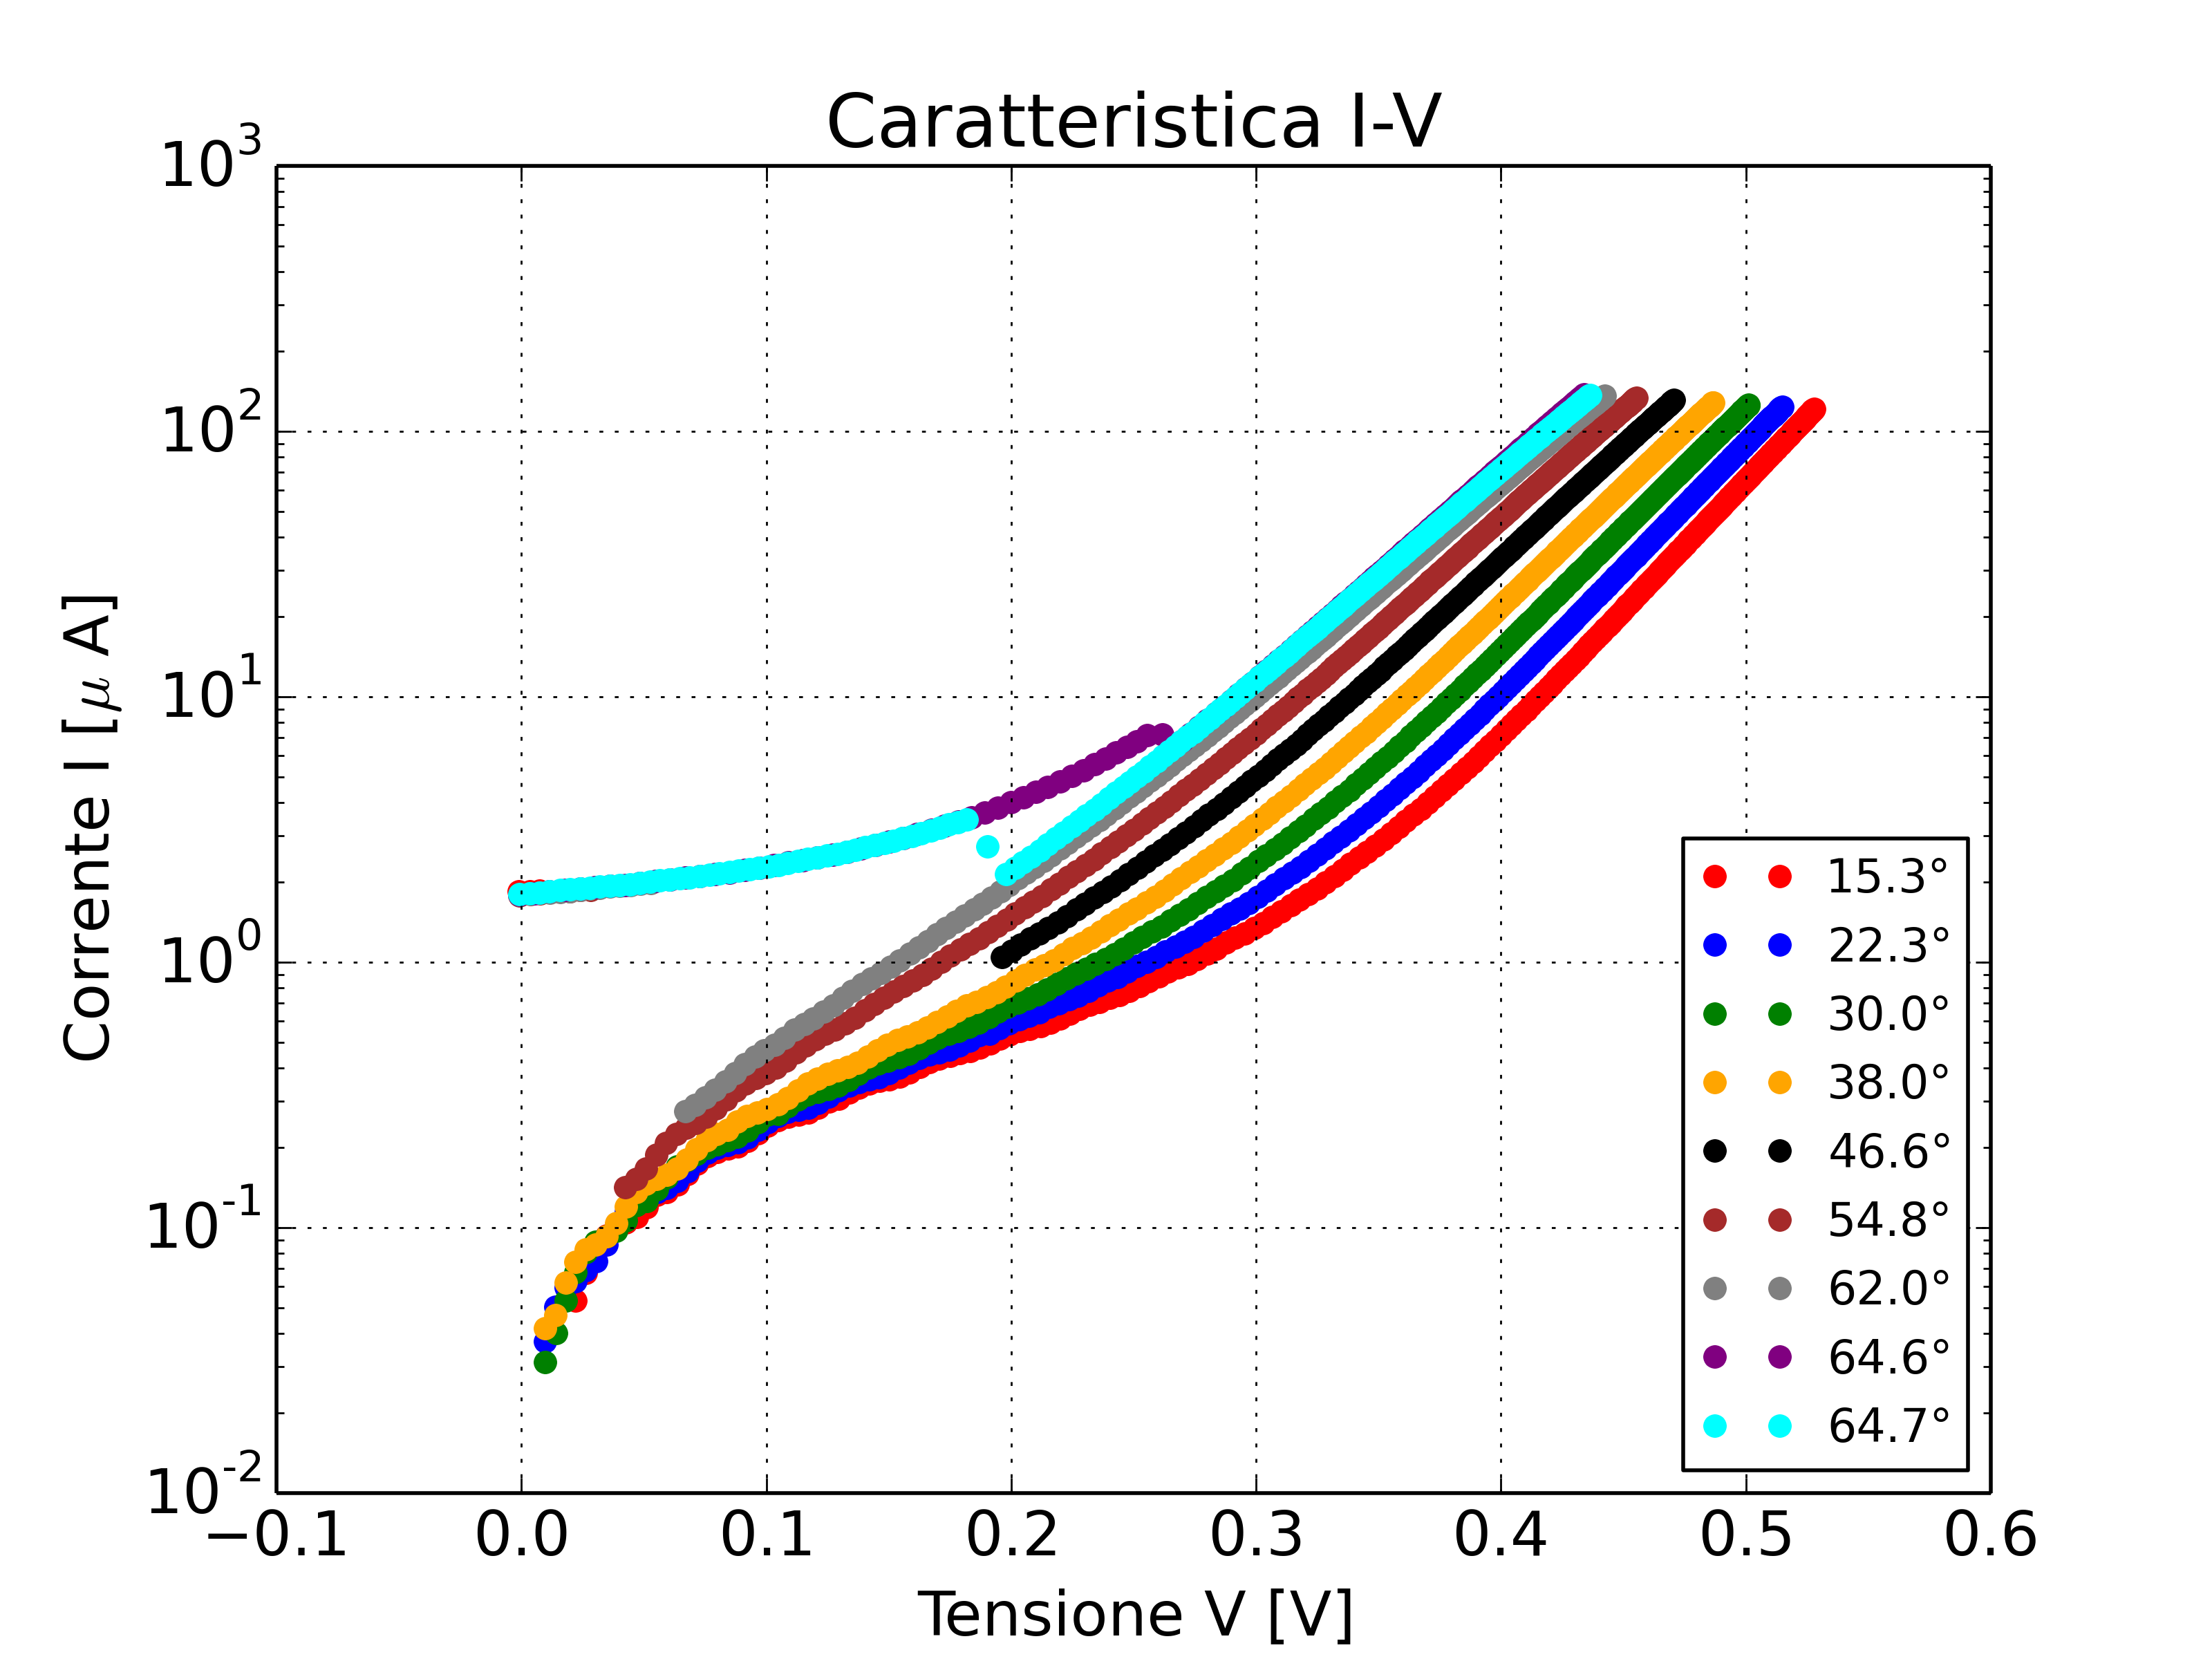
\includegraphics[width=0.7\linewidth]{./tutte_temp}
\caption{Plot delle curve I-V per alcune temperature settate.}
\label{fig:tutte_temp}
\end{figure}
  

\section{Modello di Shockley}
La prima domanda che ci poniamo è se il modello esponenziale di Shockley per le giunzioni a semiconduttore riesca a spiegare bene i dati che abbiamo acquisito o se invece vi sono deviazioni significative da esso. Il modello nella sua espressione più semplice prevede una relazione fra I e V come segue:

\begin{equation}
I = A \left( exp(BV)-1 \right)
\end{equation}

dove $B = e/nKT$. Una forma meno rozza prevede la presenza di un ulteriore parametro additivo $C$ che fisicamente rappresenta la \textit{bias current}.

\begin{equation}
I = A \left( exp(BV)-1 \right) + C
\end{equation}

Consideriamo la temperatura (effettiva) di 46.6°C e proviamo dunque a fittare entrambi i modelli appena riportati. Utilizziamo un range di correnti in cui non si arriva a valori troppo elevati, vale a dire 1-120 $\mu$A, circa, in cui siano visibili gli effetti di tutti i termini dell'equazione di Shockley. Gli errori sulle correnti sono stati posti pari a $\sigma_I = 0.05 \mu$A, (due-tre volte maggiore della sensibilità nominale della strumentazione), quelli sulle tensioni pari a $\sigma_V = 0.3$mV.\\
Per il fit di Shockley-2 (a due parametri), i risultati ottenuti sono:

\begin{table}[h]
\centering
\begin{tabular}{c|c|l}
 \textbf{A} [$\mu$A] & \textbf{B} [$V^{-1}$] & $\chi_{rid}^2$\\ 
\hline 0.01359(10) & 19.49(1) & 5.5 \\ 
\end{tabular} 
\end{table}
~\\

Per il fit di Shockley-3 abbiamo invece:

\begin{table}[h]
\centering
\begin{tabular}{c|c|l|l}
 \textbf{A} [$\mu$A] & \textbf{B} [$V^{-1}$] & \textbf{C} [$\mu$A]  & $\chi_{rid}^2$\\ 
\hline 0.01314(11) & 19.56(2) & 0.18(4) & 5 \\
\end{tabular} 
\end{table}
~\\

Nelle Figure (\ref{fig:shockley_3_pars_46gradi_semilogy},\ref{fig:shockley_3_pars_46gradi}) è riportato sia in scala semilogy che lineare il fit di Shockley-3, visualizzando solo le correnti nel range di interesse 1-120 $\mu$A. Nel grafico in scala lineare non si evidenziano dei sostanziali scostamenti dalla curva di fit dei dati sperimentali per correnti inferiori alla decina di $\mu$ A, che invece sono ben visibili in scala semilog.\\

\begin{figure}
\centering
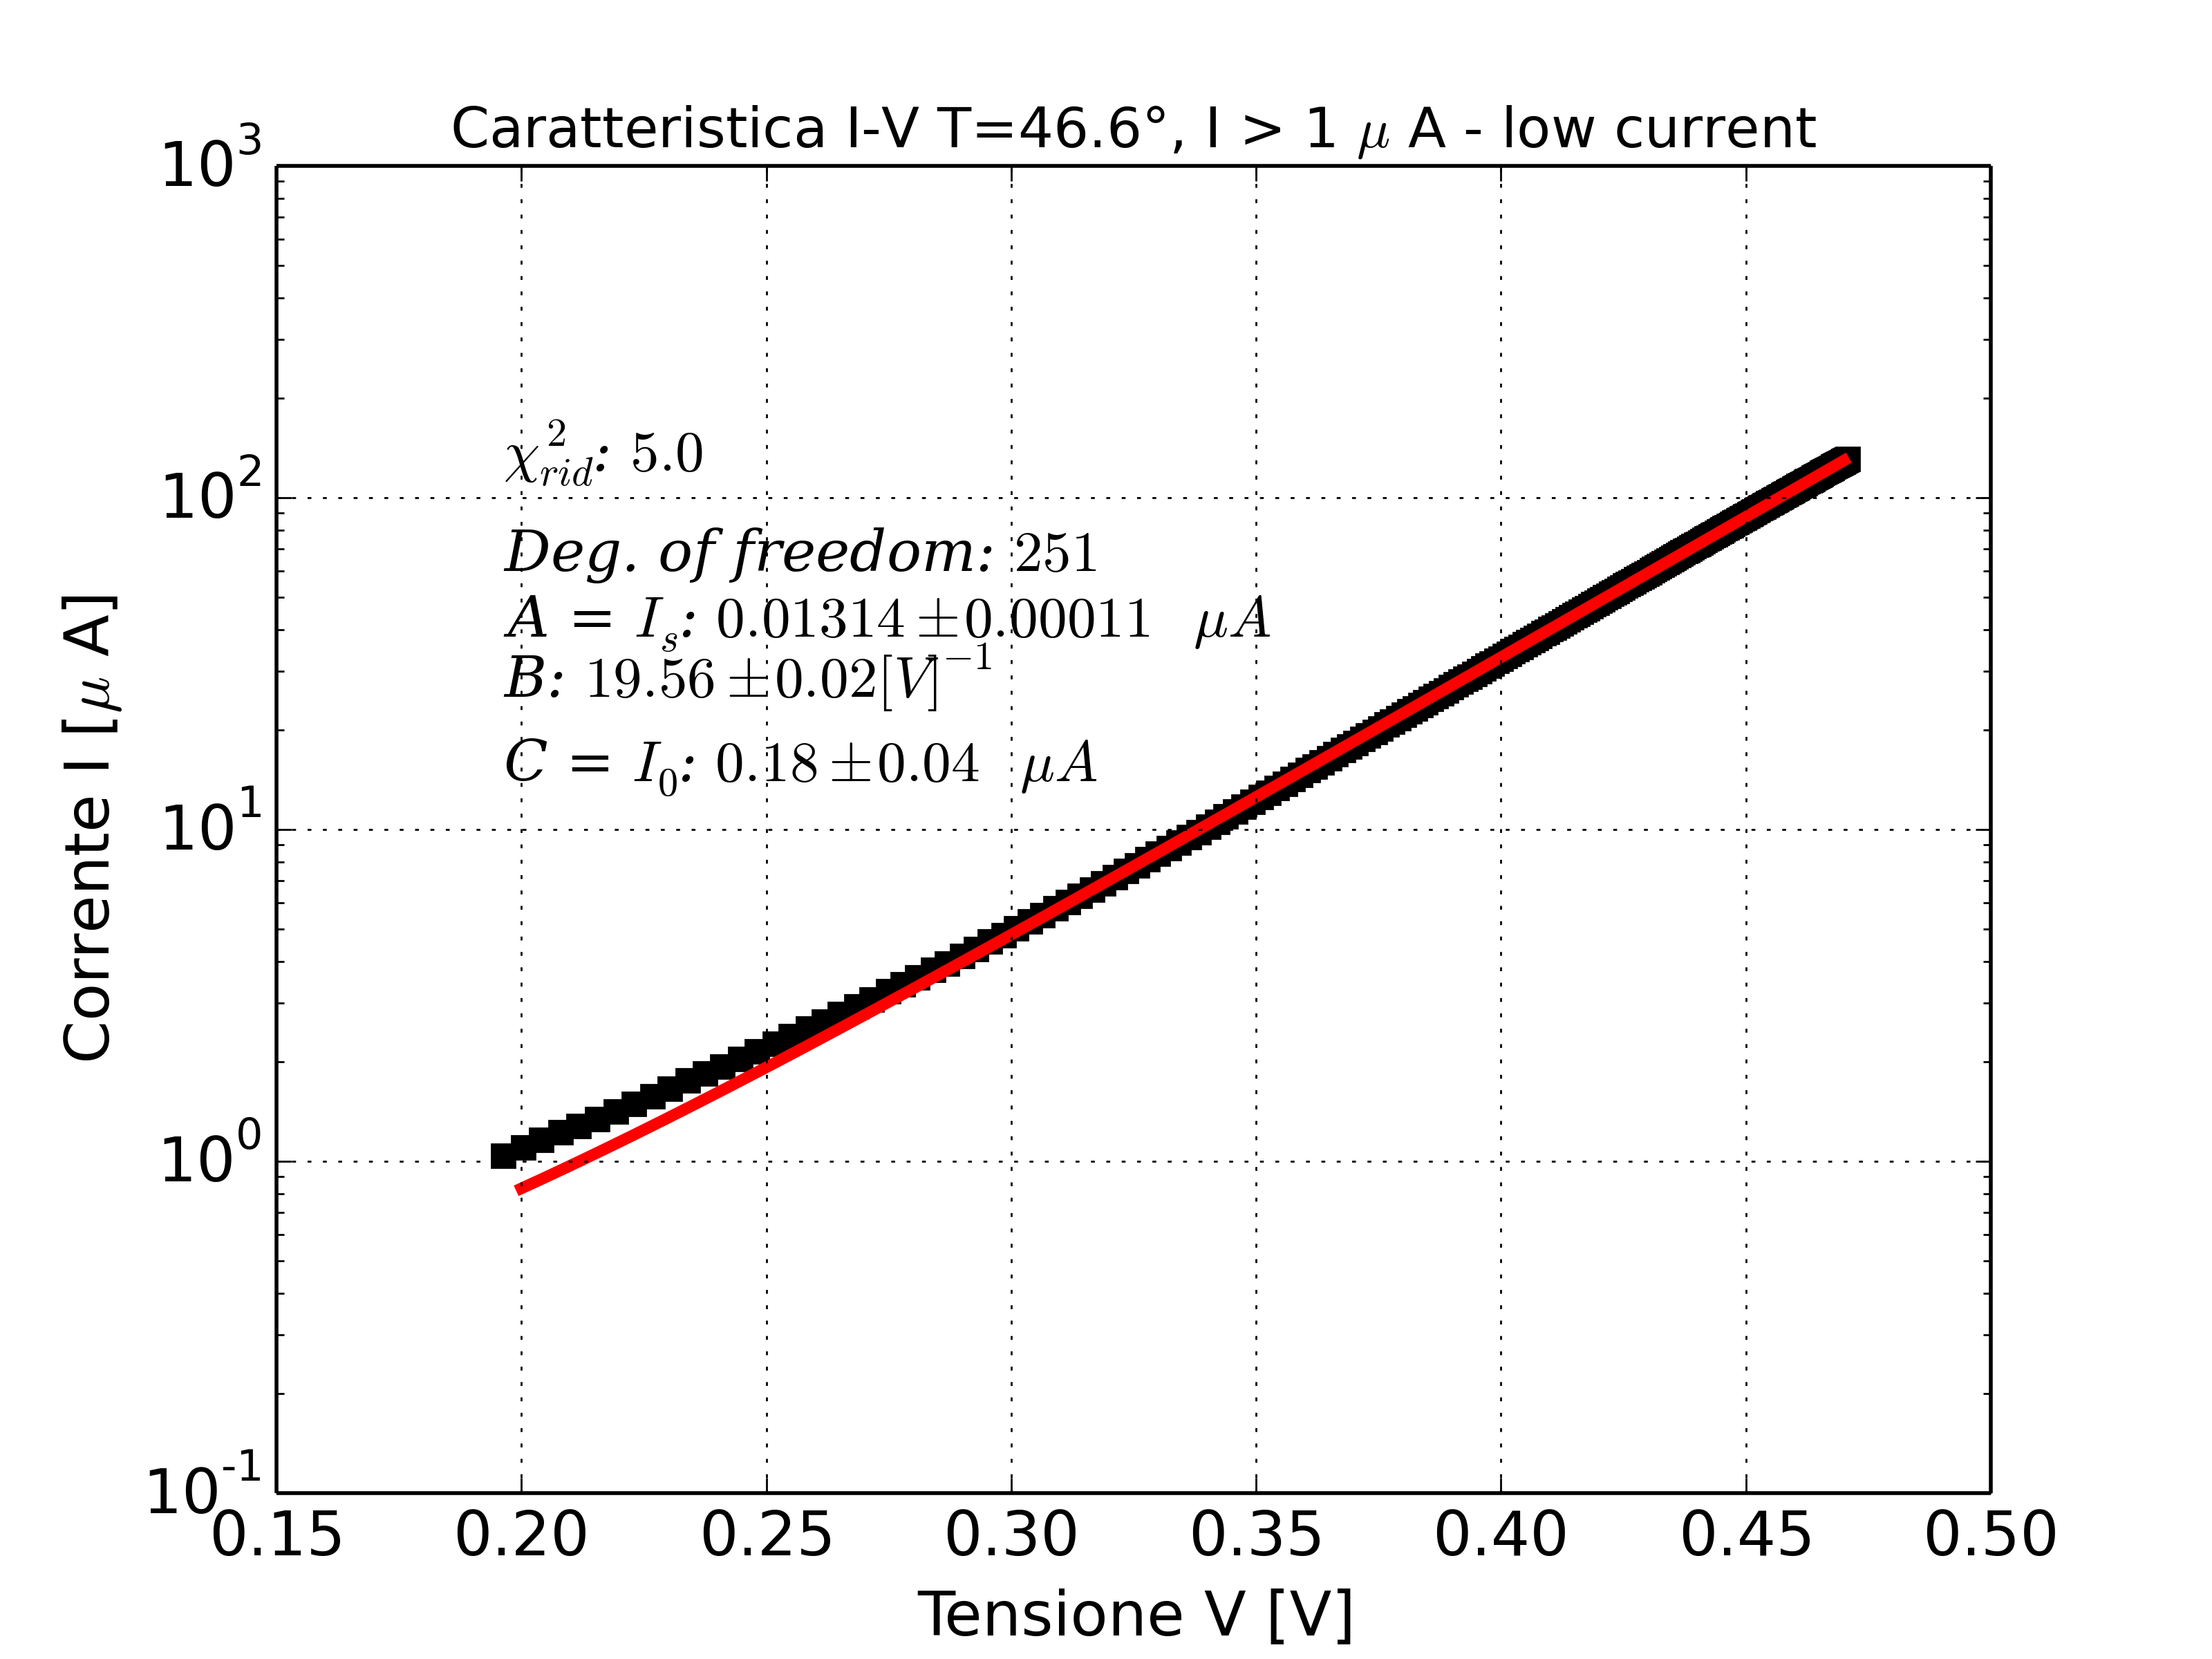
\includegraphics[width=0.9\linewidth]{./shockley_3_pars_46gradi_semilogy}
\caption{Fit di Shockley-3 semilogy: correnti nel range 1-120 $\mu$A}
\label{fig:shockley_3_pars_46gradi_semilogy}
\end{figure}

\begin{figure}
\centering
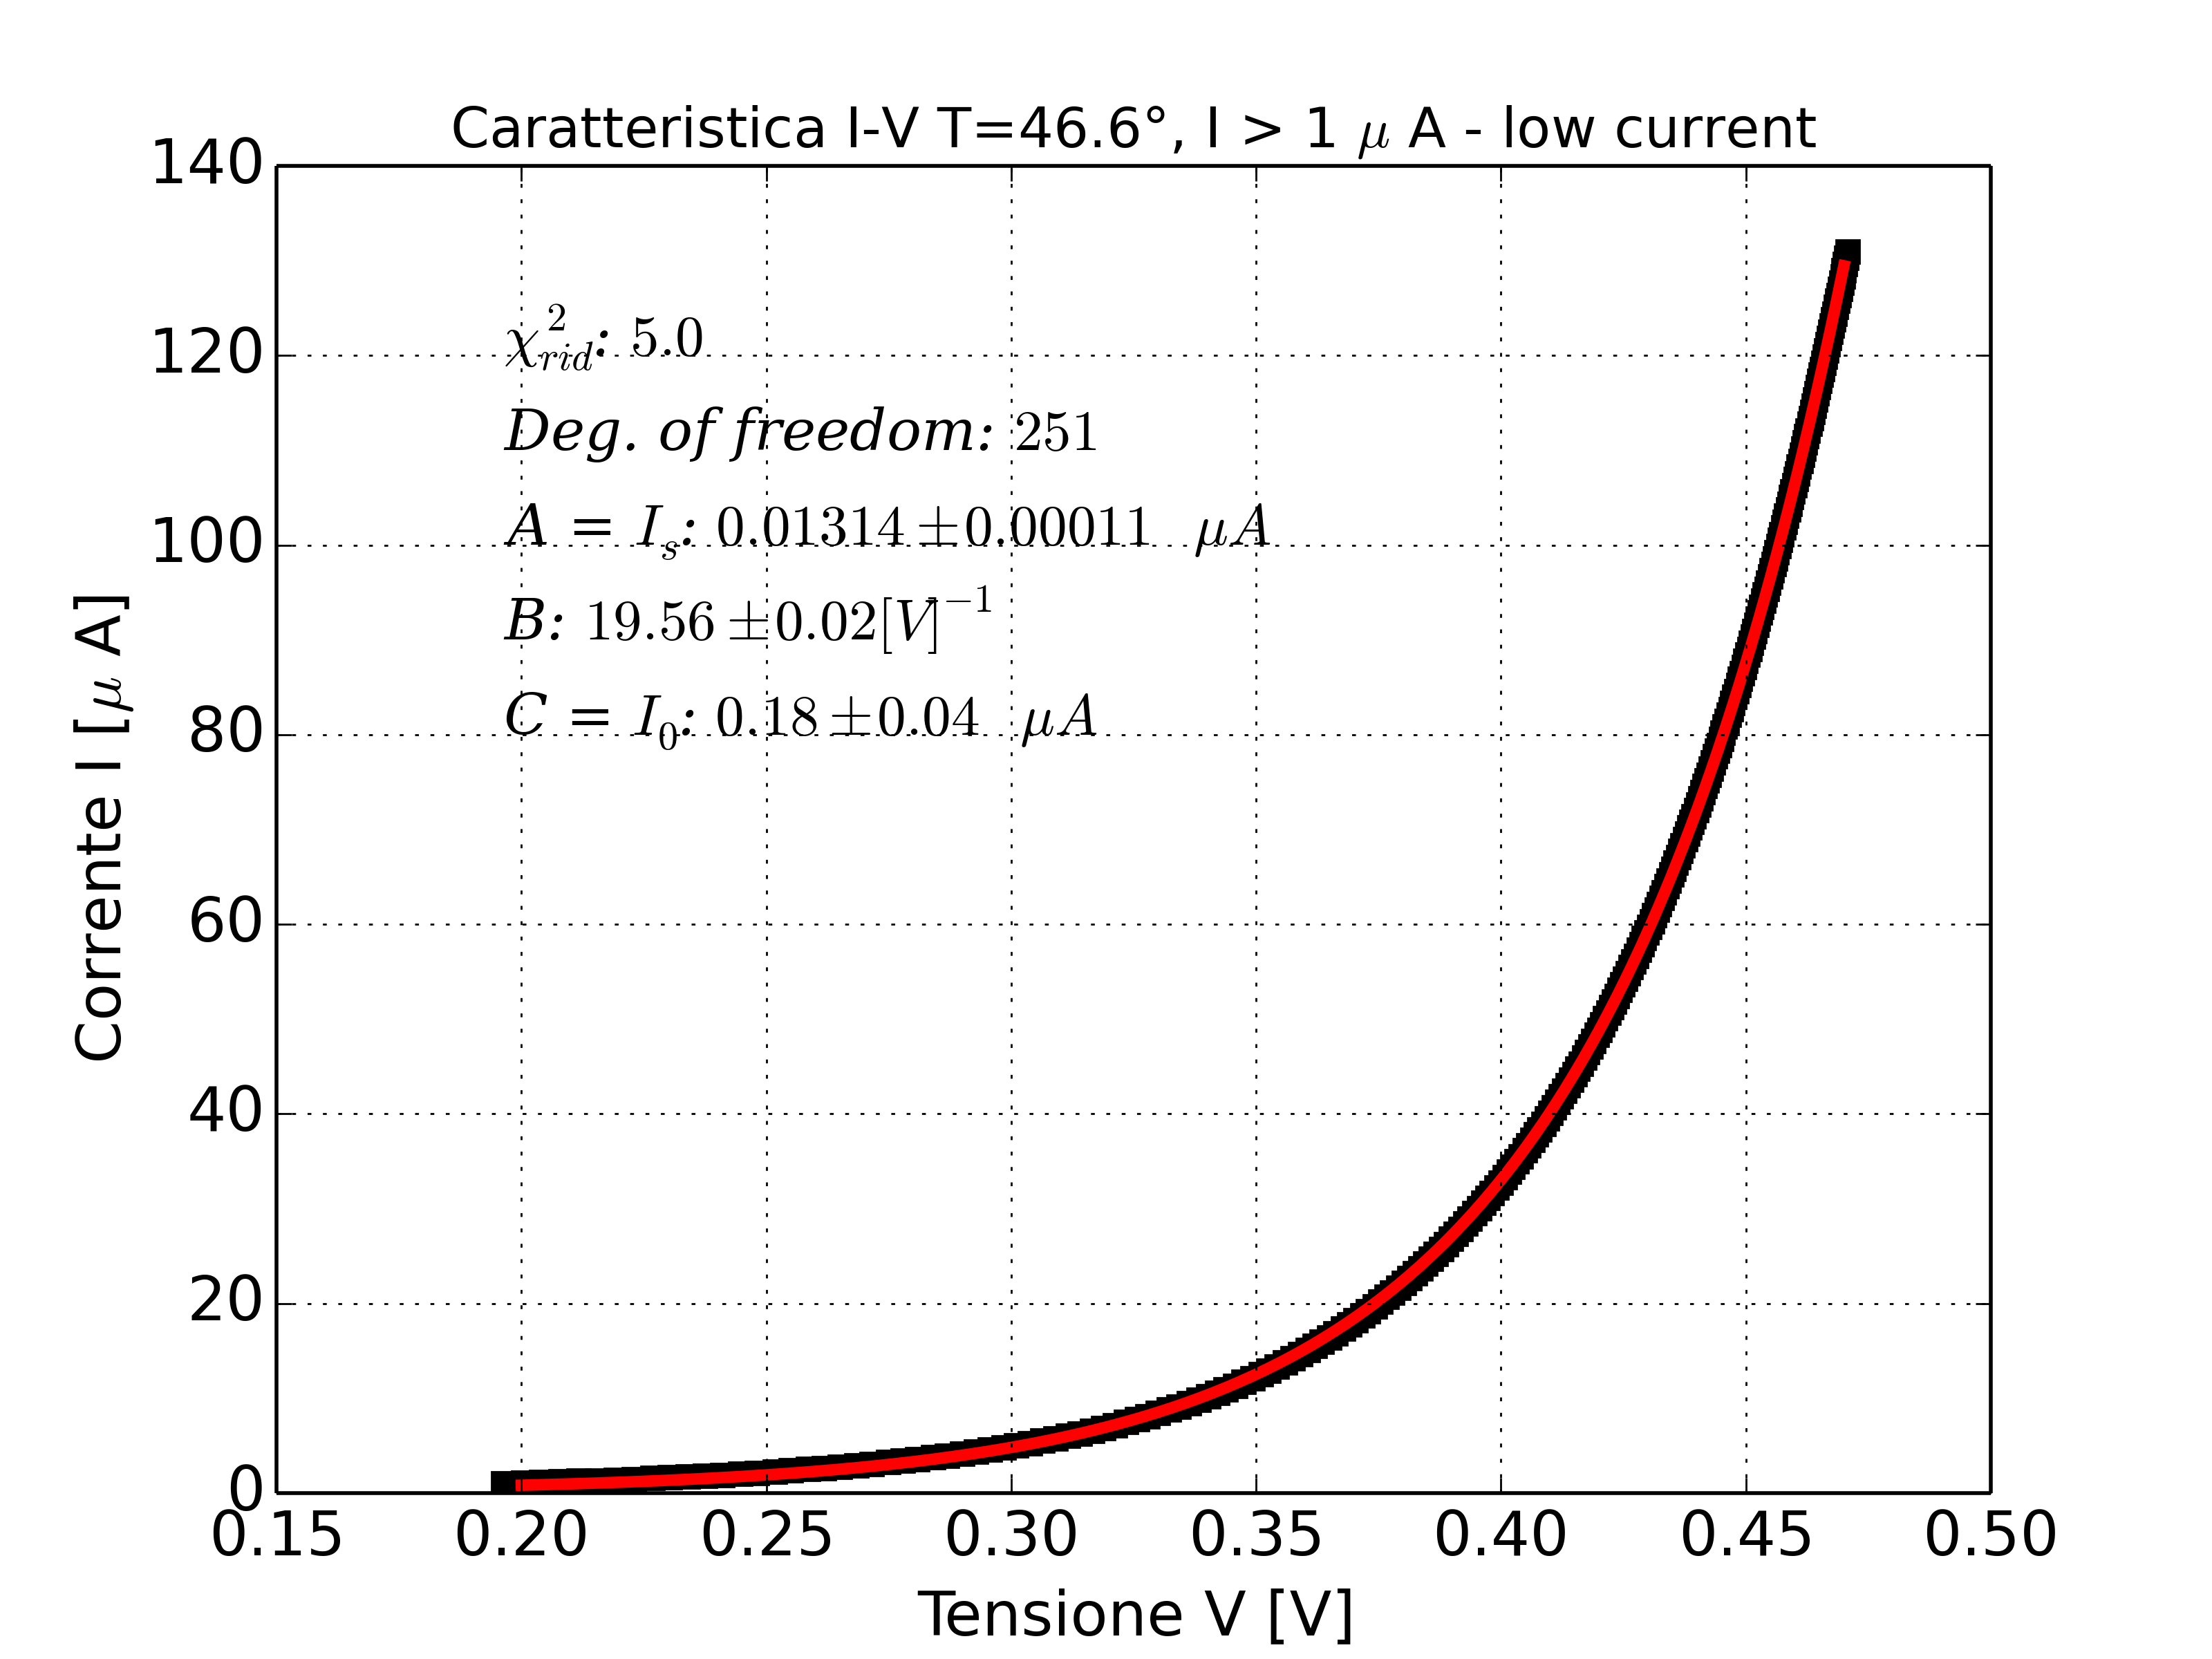
\includegraphics[width=0.9\linewidth]{./shockley_3_pars_46gradi}
\caption{Fit di Shockley-3 lineare: correnti nel range 1-120 $\mu$A}
\label{fig:shockley_3_pars_46gradi}
\end{figure}

Plottiamo ora le stesse funzioni di fit, sovrapponendole però al range completo delle correnti a nostra disposizione per verificare la validità del modello in uso su una più larga scala. Nello stesso grafico di Figura (\ref{fig:shockley_46_6_fullcur_visualiz}) sono riportate (con colori diversi) entrambe le curve di Shockley.

\begin{figure}
\centering
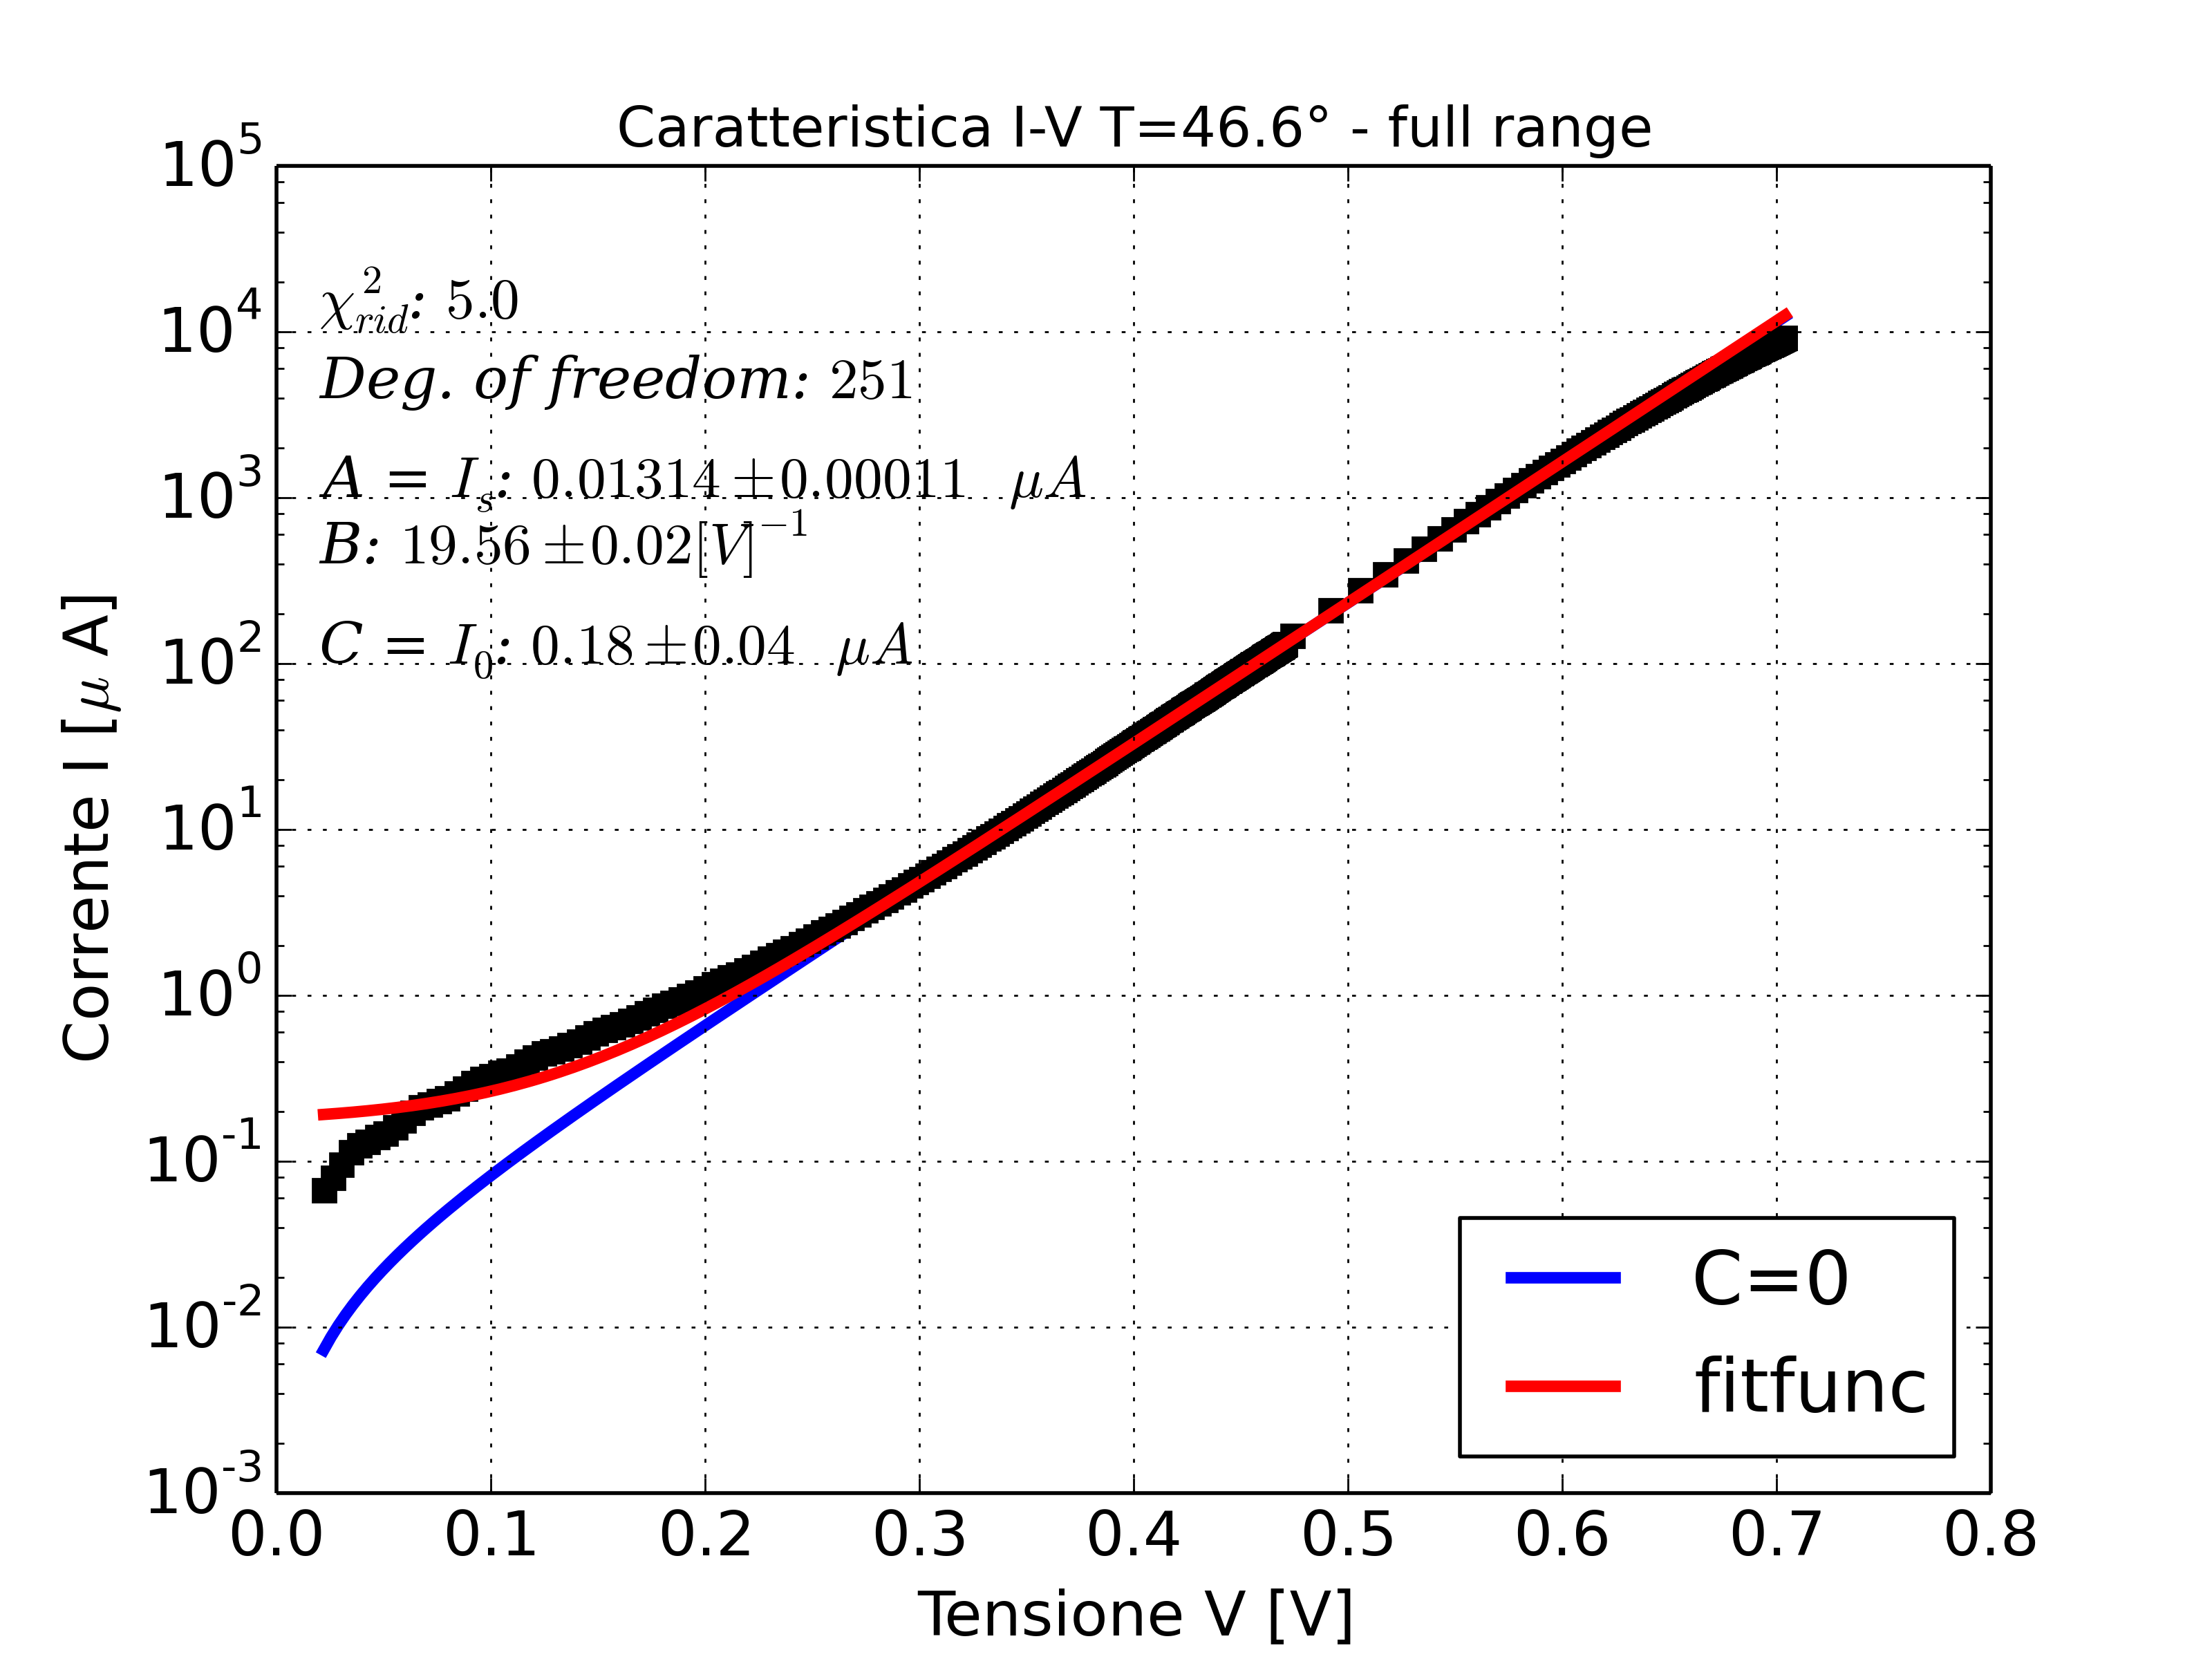
\includegraphics[width=0.9\linewidth]{./shockley_46_6_fullcur_visualiz}
\caption{Curve di fit Shockley-2 e Shockley-3 sovrapposte all'intero range di correnti.}
\label{fig:shockley_46_6_fullcur_visualiz}
\end{figure}


\section{Deviazioni dal modello di Shockley}

Come è evidente dal fit riportato in Figura (\ref{fig:shockley_3_pars_46gradi_semilogy}) e relativo ad un range di correnti 0.1-100 $\mu$A, il modello esponenziale di Shockley produce un buon accordo con i dati sperimentali solo per correnti dell'ordine di decine di $\mu$A: per valori più bassi, il fit di Shockley a due parametri sottostima anche di un ordine di grandezza $I$, mentre per correnti maggiori di $10^3-10^4 \mu$A queste sono sovrastimate (vedi Figura (\ref{fig:shockley_46_6_fullcur_visualiz})).\\
I fenomeni che possono spiegare questi comportamenti sono essenzialmente due. Ad alte correnti potrebbero iniziare ad essere rilevanti dei comportamenti ohmici della struttura che ospita la giunzione, per cui, a parità di fem, la differenza di potenziale applicata ai capi di quest'ultima è inferiore (quindi correnti inferiori). In regime di basse correnti, invece, possiamo supporre che si evidenzi come un collegamento in parallelo rispetto al diodo, attraverso il quale scorre una quantità di carica paragonabile a quella che passa nella giunzione.\\

Una modellizzazione che tenga conto di questi due fenomeni è la seguente:

\begin{equation}\label{corrente_totale}
I = I_p + I_J = GV + I_S \left[exp(B(V-R_s I_J)-1))\right]
\end{equation}

e il corrispettivo schema circuitale è in Figura (\ref{fig:schema_circuit}).\\

\begin{figure}
\centering
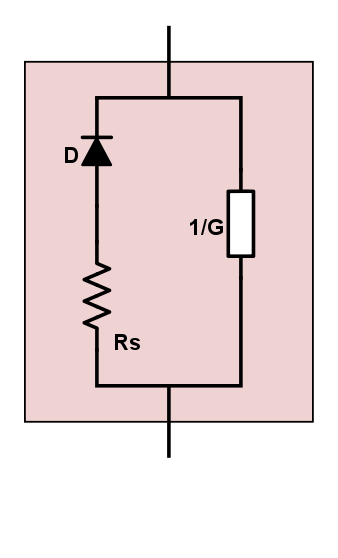
\includegraphics[width=0.3\linewidth]{./schema_circuit}
\caption{Schema circuitale del modello "reale" presentato}
\label{fig:schema_circuit}
\end{figure}


Con $G$ indichiamo il reciproco della resistenza parallela equivalente, con $I_J$ la corrente che scorre nella giunzione, $R_s$ è la resistenza in serie alla giunzione stessa. Un buon fit dei dati dovrà, quindi, tenere conto contemporaneamente dell'influenza del ramo in parallelo, visibile a basse correnti, e della resistenza in serie, che si evidenzia ad alte $I$.\\

Un modo per considerare allo stesso tempo questi due fattori è quello di ricorrere ad una procedura iterativa su tutti i dati di corrente e che, ottimisticamente, converga a dei valori accettabili dei parametri $G$, $R_s$, $I_S$, $B$.

\section{Procedura iterativa di fit}
La procedura iterativa si basa, essenzialmente, su di una serie di passaggi che di volta in volta migliorano le stime dei parametri ottenuti nei passi precedenti. In particolare:

\begin{enumerate}

\item Come prima stima del parametro G, implementiamo un fit lineare sui dati a basse correnti ($I \lesssim 1 \mu$A) del tipo $I = GV$. Si rimanda alla sezione () per alcune annotazioni su questo passo.

\begin{lstlisting}
g_0, pcov_lin = optimize.curve_fit(linfit, 
xdata[:argmax(ydata>=1)], ydata[:argmax(ydata>=1S)], p0lin, sigmay)
\end{lstlisting}

\item INIZIO LOOP: Con la stima di $G^{i=0}$ possiamo ottenere un primo valore della corrente che scorre nella giunzione $I_J = I - G^i V$.

\begin{lstlisting}
jun_cur = ydata - g_0*xdata
\end{lstlisting}

\item Per regimi di correnti non troppo alti, il primo termine nella (\ref{corrente_totale}) è trascurabile rispetto al comportamento esponenziale. La relazione si può dunque riscrivere come:

\begin{equation}
V(I=I_J) = \frac{1}{B} log \left(\frac{I}{I_J} + 1 \right) + R_s I
\end{equation}

Fittiamo ora questa funzione esplicita di $I_J$ per ottenere la prima stima dei tre parametri rimasti $I_S^i$, $R_s^i$, $B^i$.

\begin{lstlisting}
p_loop, pcov_loop = optimize.curve_fit(tension_junc, 
abs(jun_cur[argmax(jun_cur>=sup_current):]), 
xdata[argmax(jun_cur>=sup_current):], p0_loop, sigmax)
\end{lstlisting}


\item Avendo ottenuto i parametri $I_S^i$, $R_s^i$, $B^i$, possiamo impiegarli risolvendo a ritroso l'equazione precedente e trovare così i valori aggiornati della corrente di giunzione $I_{J}^{i+1}$. La risoluzione questa volta è numerica, dato che l'espressione in funzione di $I_J$ è in forma implicita, e per implementarla usiamo la routine \textsc{fsolve} di Python:

\begin{lstlisting}
def fitsolve(I_j, I_s, B, R, v):
    return v - log(abs(I_j)/abs(I_s) + 1)/B + I_j*R*10**(-6)
jun_cur_1 = optimize.fsolve(fitsolve, jun_cur, (I_S, B, R_s, xdata) );
\end{lstlisting}

\item A partire dal nuovo array $I_{J}^{i+1}$ calcoliamo $I^{i+1} = G^i V + I_{J}^{i+1}$

\begin{lstlisting}
tot_cur = g_0*xdata + jun_cur_1
\end{lstlisting}

\item Similmente al passo introduttivo al loop, volendo cercare una correzione al parametro $G^i$, possiamo fittare la differenza fra i dati sperimentali $I$ e $I^{i+1}$, con la funzione: $I - I^{i+1} = \delta G \; V$, e il nuovo valore $G^{i+1}$ sarà quindi dato da $G_{i+1} = G^i +\delta G$. Anche in questo caso, i valori di correnti che andremo a selezionare per il fit saranno solo quelle al di sotto della nostra soglia di 1$\mu$A.

\begin{lstlisting}
delta_g, delta_g_pcov = optimize.curve_fit(linfit, xdata[:argmax(tot_cur>=1)],
ydata[:argmax(tot_cur>=1)]-tot_cur[:argmax(tot_cur>=1)], g_0, sigmay);

g_1 = g_0 + delta_g
\end{lstlisting} 

\item FINE LOOP: come ultimo passo prima di chiudere il loop, è necessario confrontare i parametri (i+1) con quelli (i) e definire un qualche criterio di convergenza. Quello da noi individuato, in seguito a diversi tentativi, è verificare se:

\begin{equation}
\left| X^{i+1} - X^{i}  \right| < \frac{\delta X^{i+1}}{M}
\end{equation}

con $M$ un'opportuna costante positiva maggiore di 1. Se tale condizione viene verificata contemporaneamente per tutti e 4 i parametri in gioco, allora il ciclo loop si ferma.

\end{enumerate}

\subsection{Annotazioni sul fit iterativo}
E' opportuno chiarire meglio alcuni passaggi della procedura iterativa.\\

\begin{itemize}

\item Al passo 1 (introduttivo al ciclo loop) si è verificato che la stima prodotta di $G^0$ con il fit lineare del modello $I = GV$ sui primi valori di corrente dà una stima soddisfacente, (indicativamente diciamo $G \lesssim 6-7 \mu S$) tale per cui la convergenza del parametro G nel loop si verifica, solo per temperature non superiori ai 50-60 °C. Al di sopra di questo valore il risultato della stima di G non permette la convergenza, poichè ad ogni iterazione questo aumenta in maniera monotona. In questi casi, allora, è stato ritenuto opportuno usare un modello di fit che includa sia la parte lineare che quella esponenziale: procedendo in tale modo la convergenza si è sempre verificata.


\item Al passo 3 è stata posta una condizione aggiuntiva sul range dei dati su cui fittare i parametri, e cioè che vengano prese solo le correnti (di giunzione) superiori ad un certo valore, posto arbitrariamente a 10$\mu$A. Si è osservato, nel corso di prove successive, che la convergenza, e soprattutto la stima numerica dei parametri restituiti dal fit, sembra migliore. Possiamo giustificare questo comportamento ricordandoci che questa forma funzionale è tanto più valida quanto maggiori sono le correnti in gioco, per cui la usiamo in un range opportuno di correnti di giunzione.\\

\end{itemize}

\subsection{Risultati del fit iterativo}
I risultati della procedura iterativa sono stati spesso difficili da ottenere, a causa principalmente di problemi di overflow o di valutazioni di funzioni (come ad esempio il logaritmo) per argomenti negativi, che ovviamente non erano dati in input ma erano risultati temporanei ottenuti nelle iterazioni interne agli script di ottimizzazione, per questo motivo quasi impossibili da prevedere (e da porre rimedio). Con un lavoro di fino, si è riusciti ad ottenere dei risultati piuttosto soddisfacenti dei parametri di fit, sia a livello grafico tracciando le curve di best-fit. In generale, quindi, la convergenza della procedura di fit si è ottenuta in un numero di iterazioni compreso fra 5-10.\\
Un problema evidente per alte correnti, come si vedrà dai grafici che sono riportati di seguito, è il comportamento davvero singolare della curva di fit che non si riesce a spiegare se non prendendo in considerazione dei fenomeni di non-convergenza nella routine di fit. \\
Effettivamente, andando ad esaminare in maniera dettagliata i singoli passi, questa forma poco "analitica" della curva I-V è dovuta ad una non convergenza della procedura di risoluzione numerica del passo (4) per il calcolo delle correnti di giunzione (i+1)-esime, da noi effettuata con l'algoritmo \textsc{FSOLVE}. Una riprova di ciò si ha valutando la differenza $I_{J}^{i+1} - I_{J}^{i}$, che in linea di principio dovrebbe diventare sempre più piccola all'aumentare numero di iterazioni. Nella realtà, per basse correnti la convergenza era effettivamente ottima, mentre per alte $I$ (superiori a $10^3 \mu$A) tale differenza esplodeva invariabilmente rendendo il plot della funzione di fit imprevedibile e con errori assolutamente privi di senso (infatti per valori di I circa compresi fra $10^3 - 10^4 \mu$A sono stati oscurati per questioni anche grafiche ed estetiche).\\
Si è provato a rimediare a questa situazione impiegando altre routine di risoluzione numerica degli zeri di funzioni, come \textsc{broyden1}, \textsc{broyden2} e \textsc{root} ottenendo, se possibile, risultati ancora peggiori. Probabilmente si evidenzia un problema di cattivo condizionamento di queste routine per valori di input in questo particolare range.\\
Ad ogni modo, la corrispondenza del fit con i dati sperimentali per valori di corrente piccoli e medi fino ai mA è complessivamente molto buona, come visibile dai grafici delle Figure (\ref{iterative_fit}).\\

\begin{figure}
\centering
\subfloat[]{
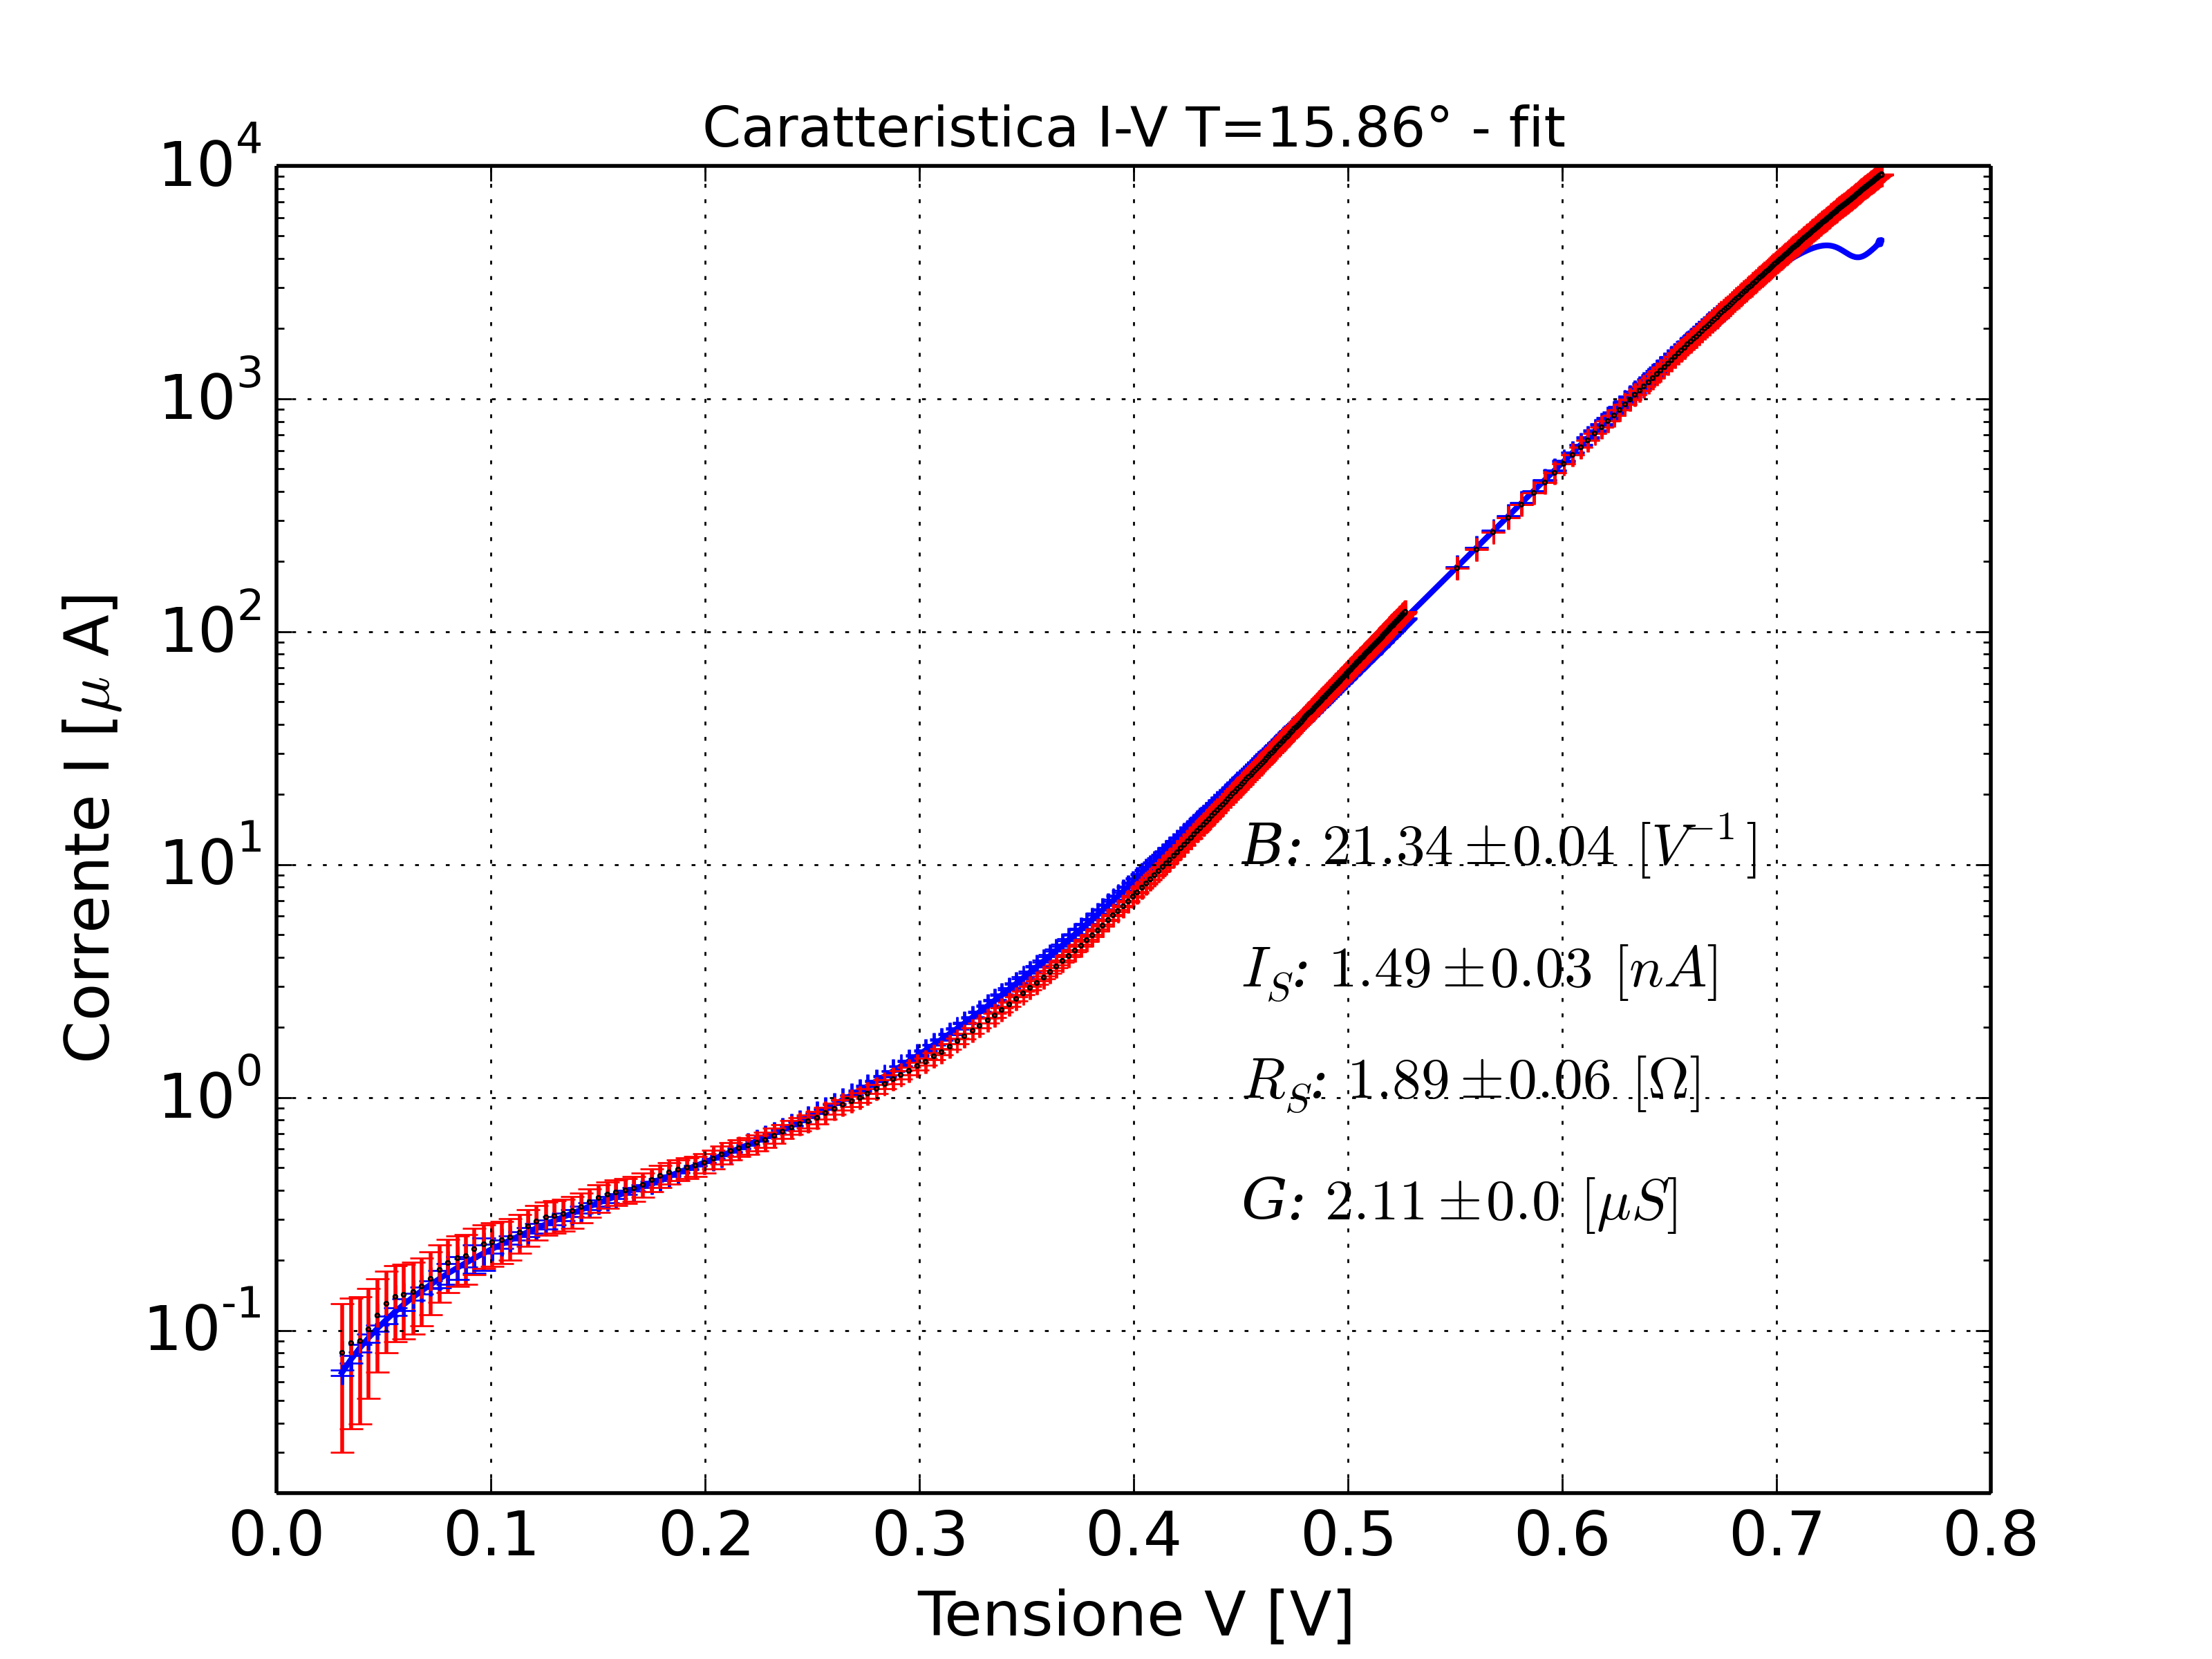
\includegraphics[width=0.5\linewidth]{./C1}}
\subfloat[]{
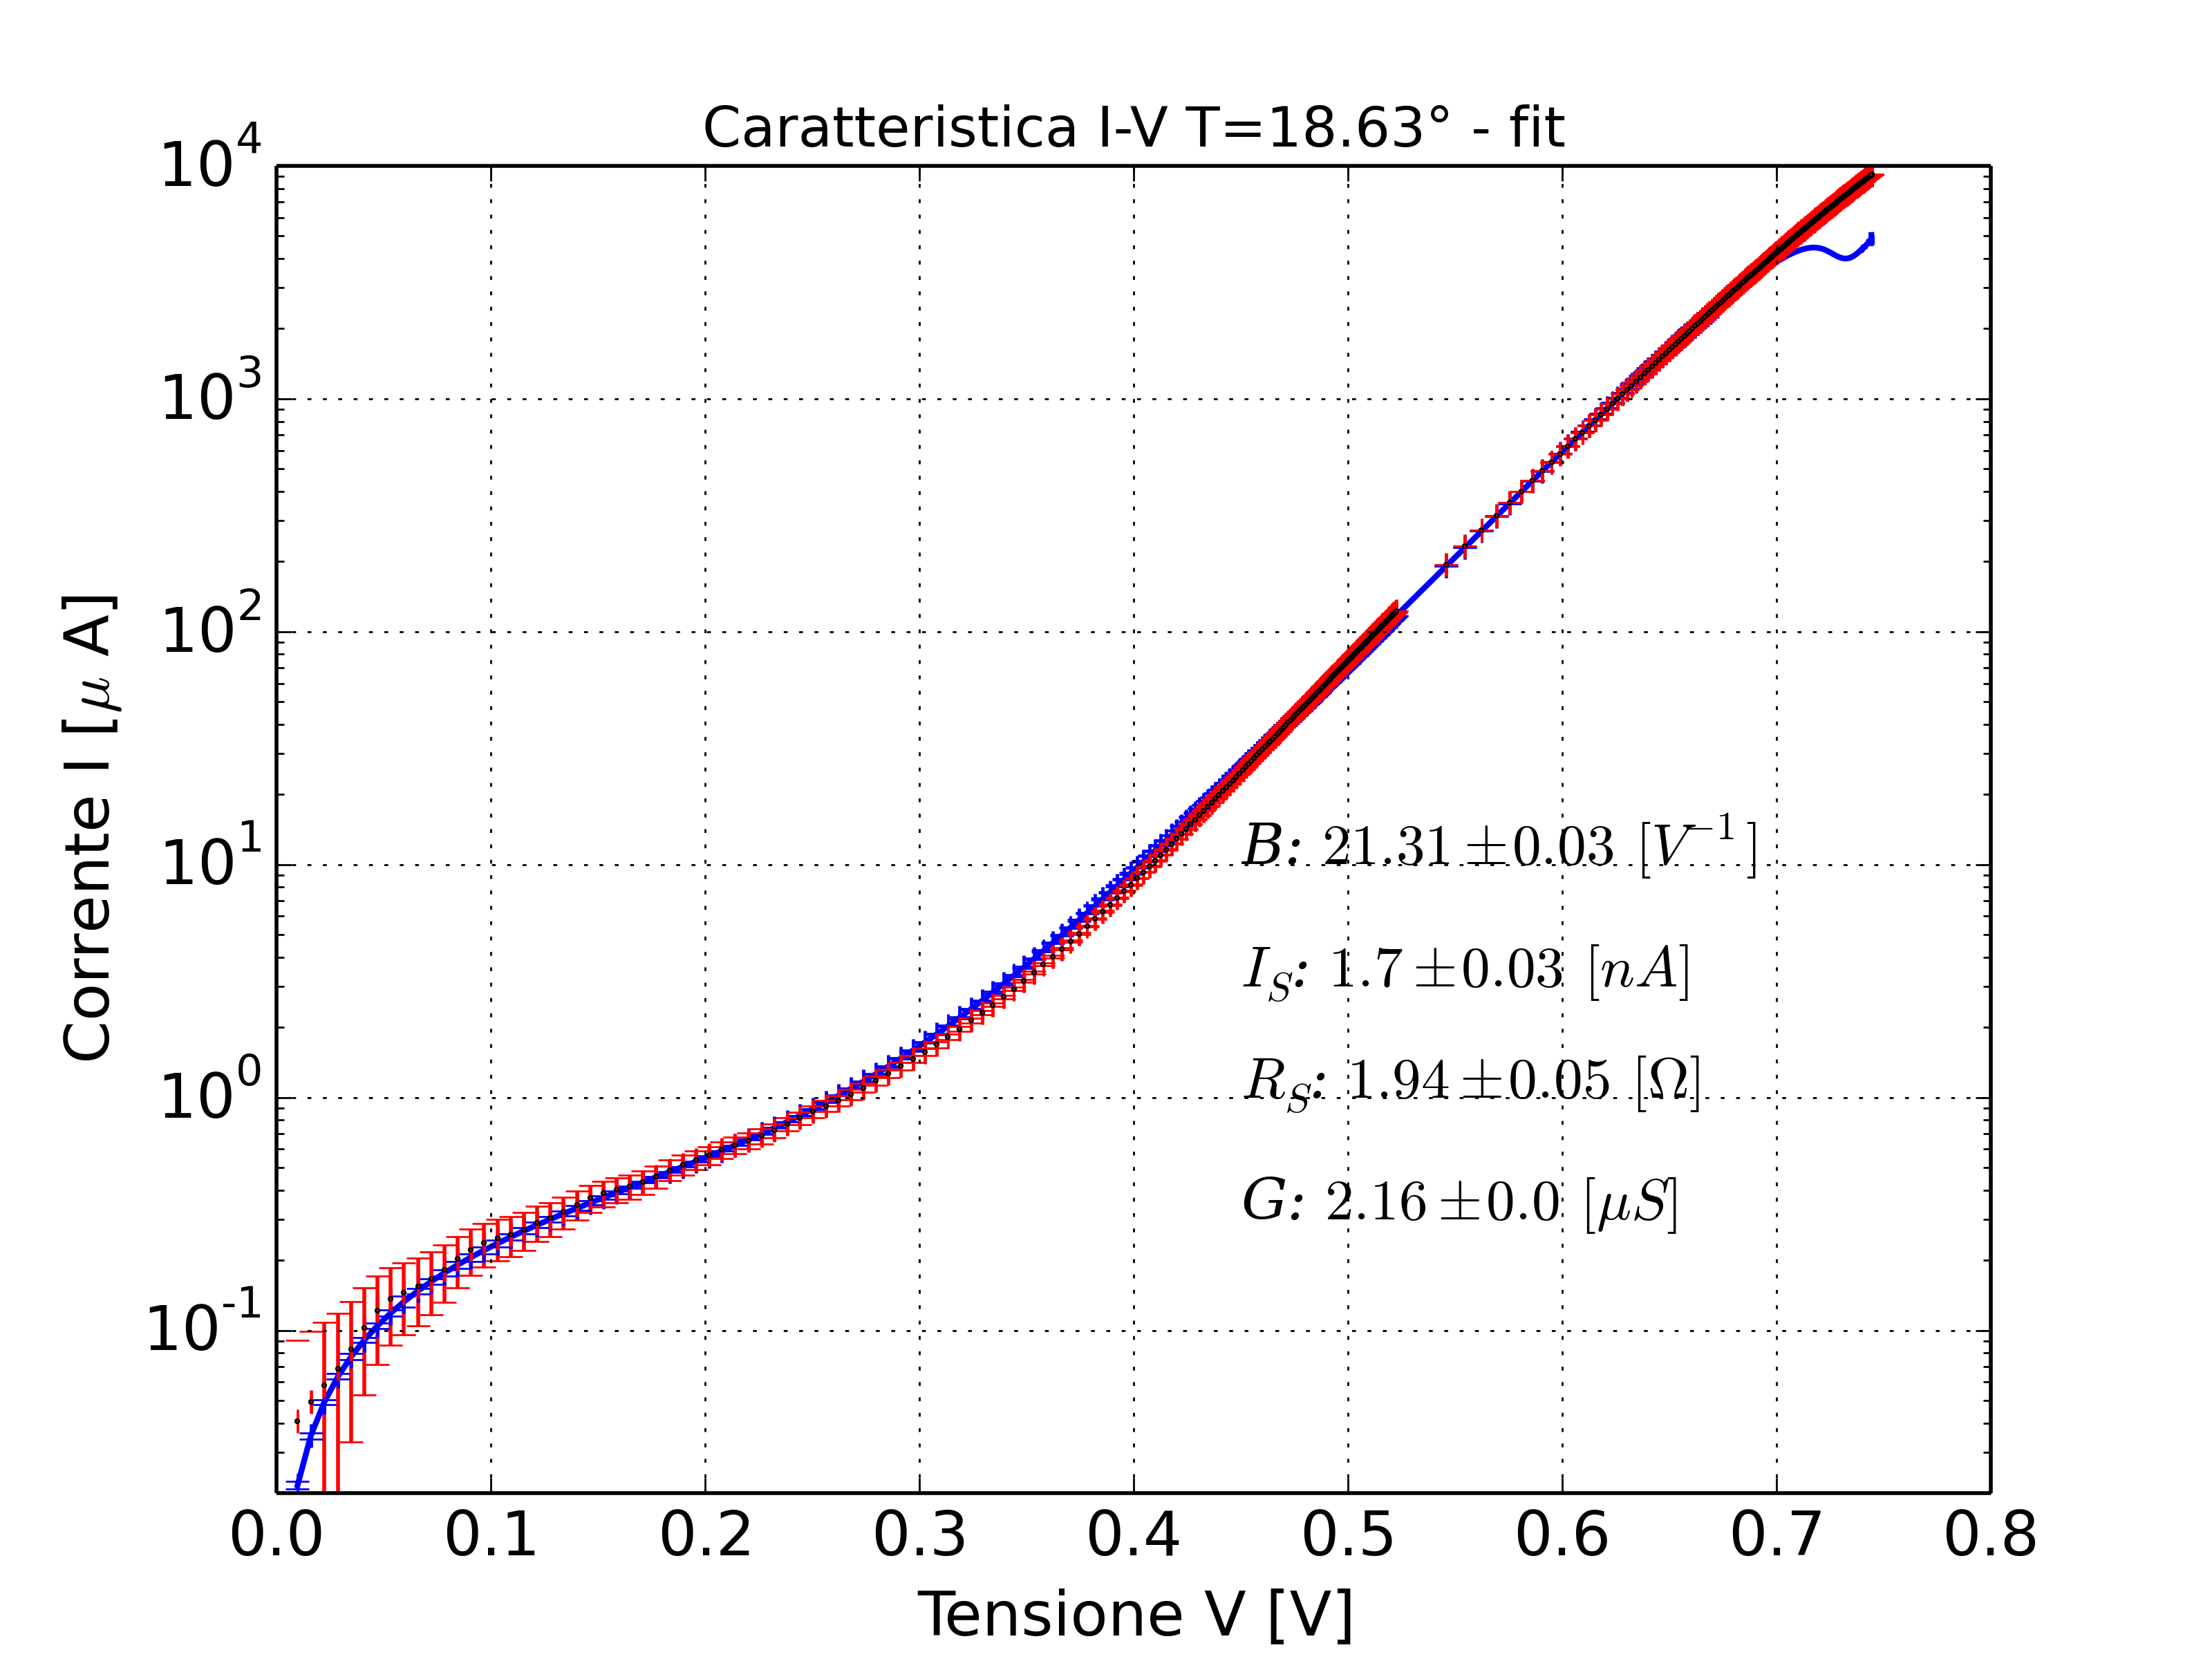
\includegraphics[width=0.5\linewidth]{./C2}}
\qquad
\subfloat[]{
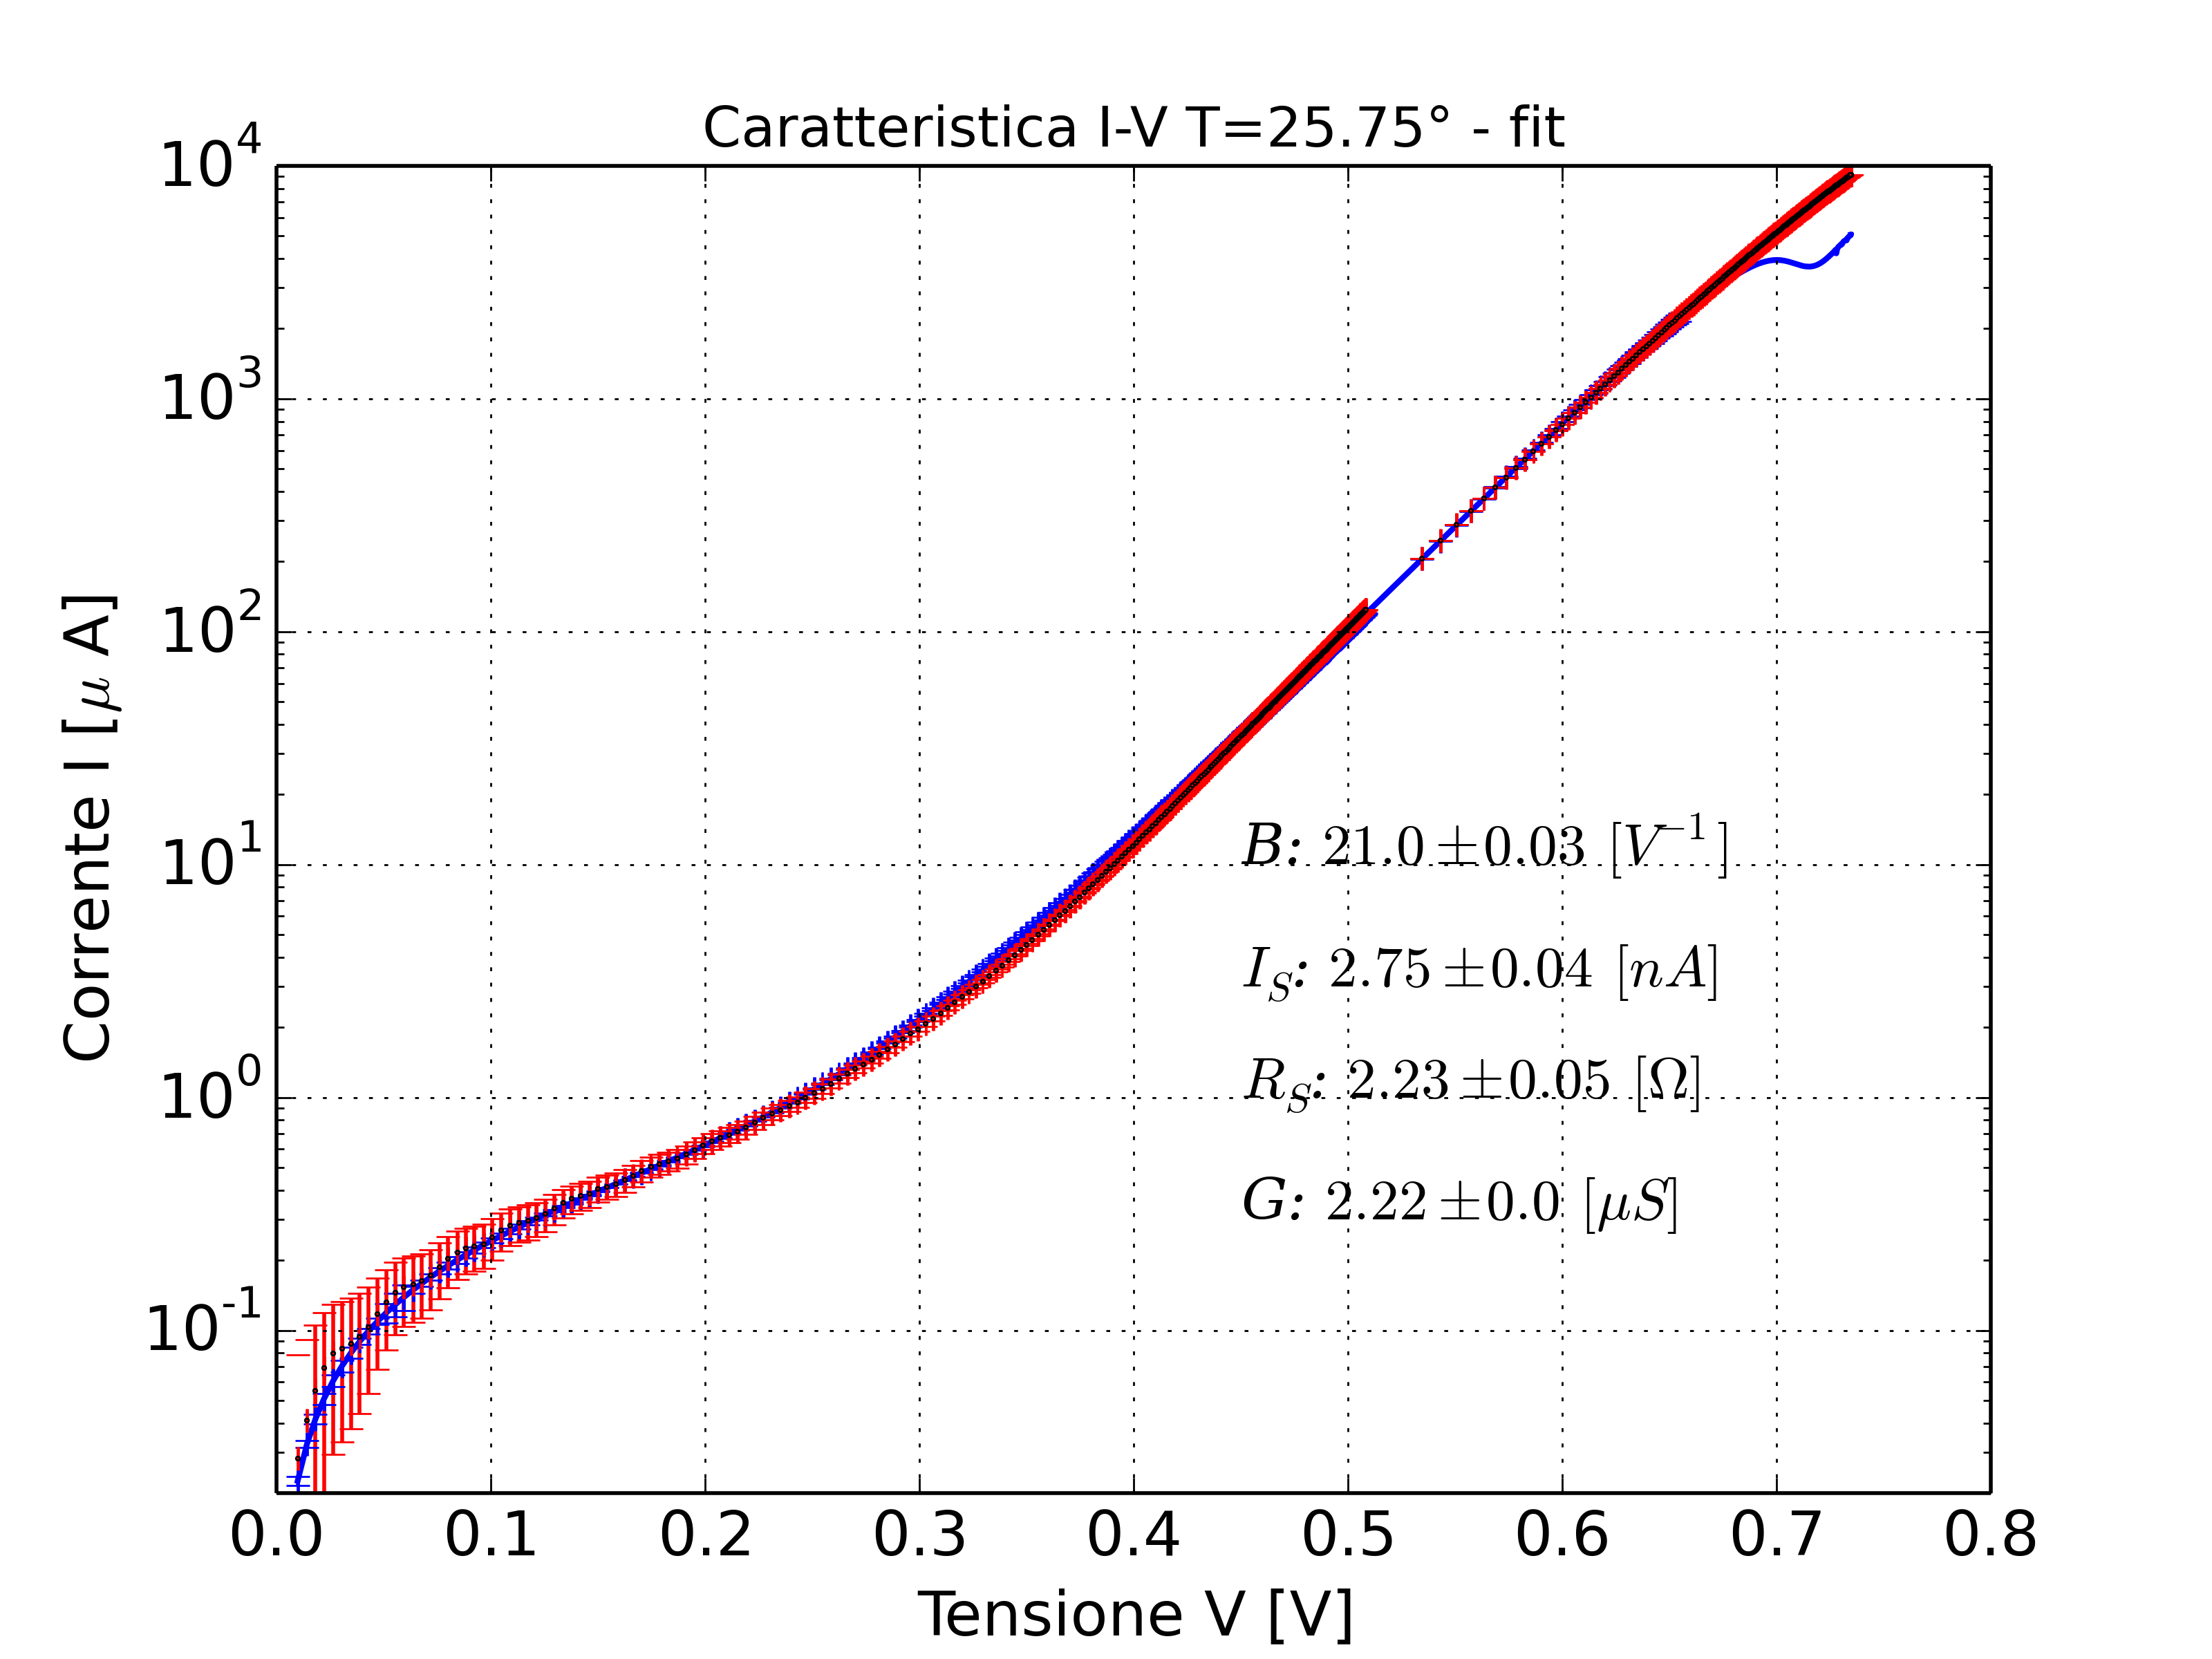
\includegraphics[width=0.5\linewidth]{./C3}}
\subfloat[]{
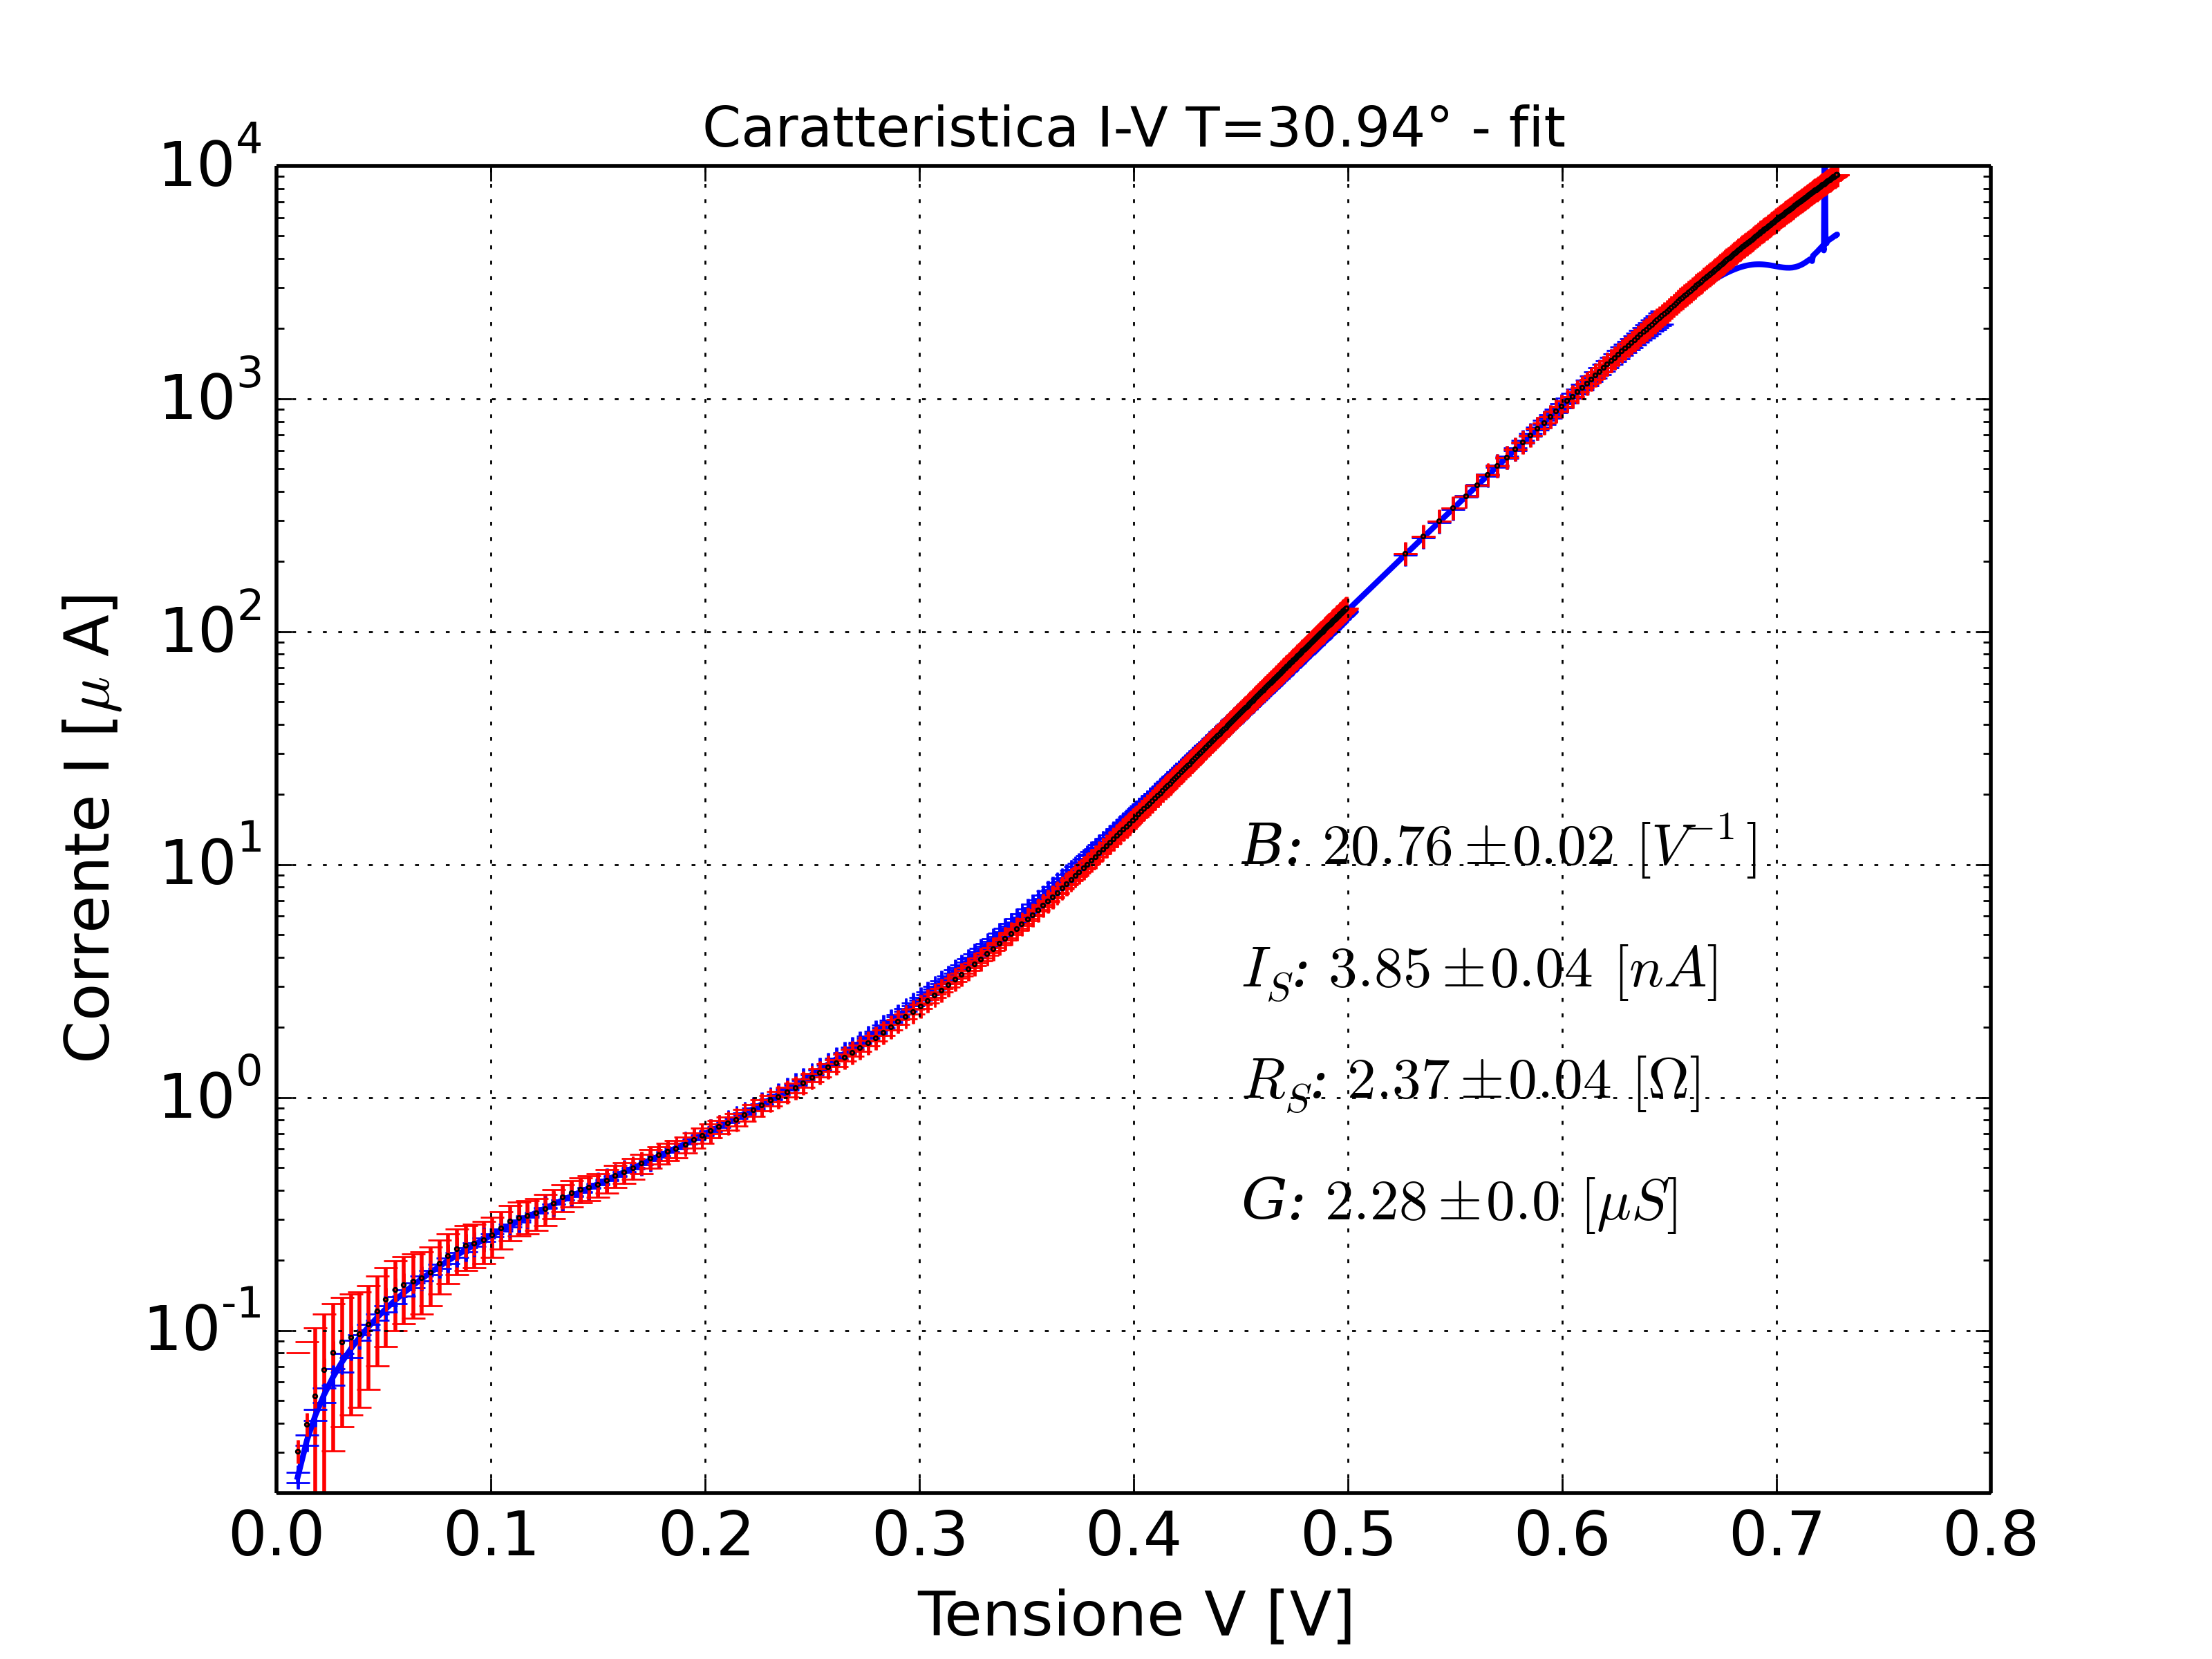
\includegraphics[width=0.5\linewidth]{./C4}}
\qquad
\subfloat[]{
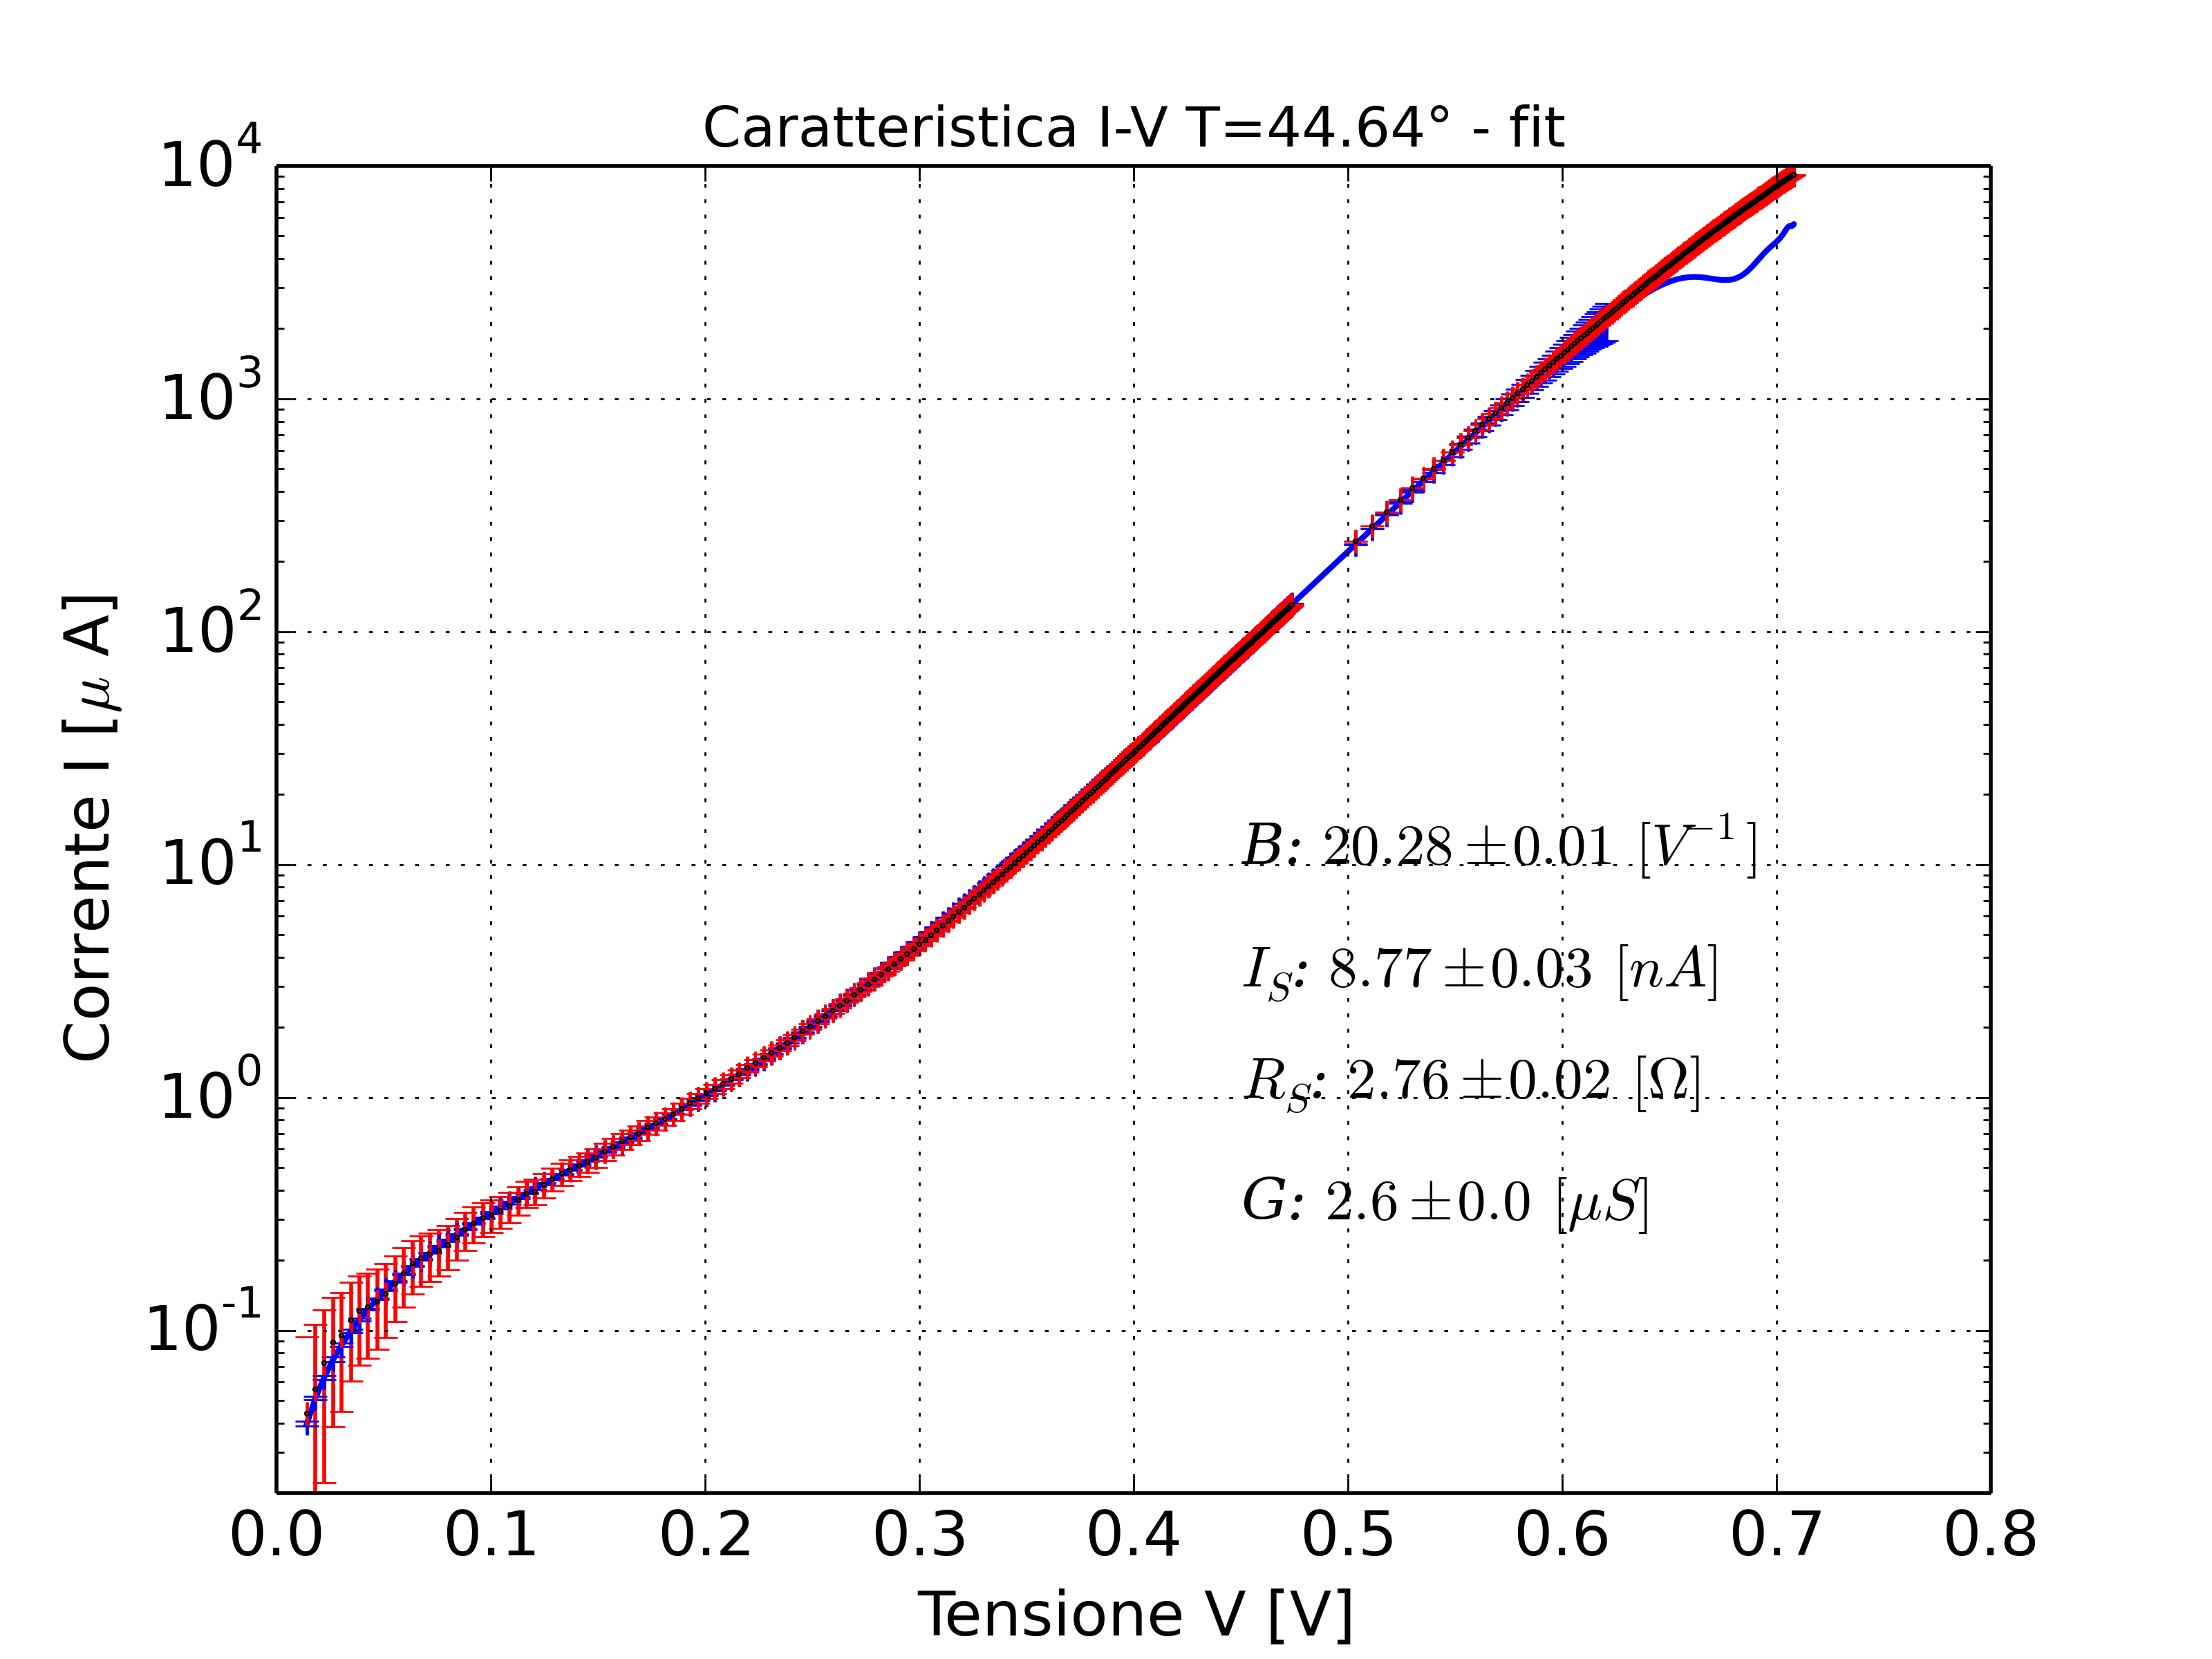
\includegraphics[width=0.5\linewidth]{./C8}}
\subfloat[]{
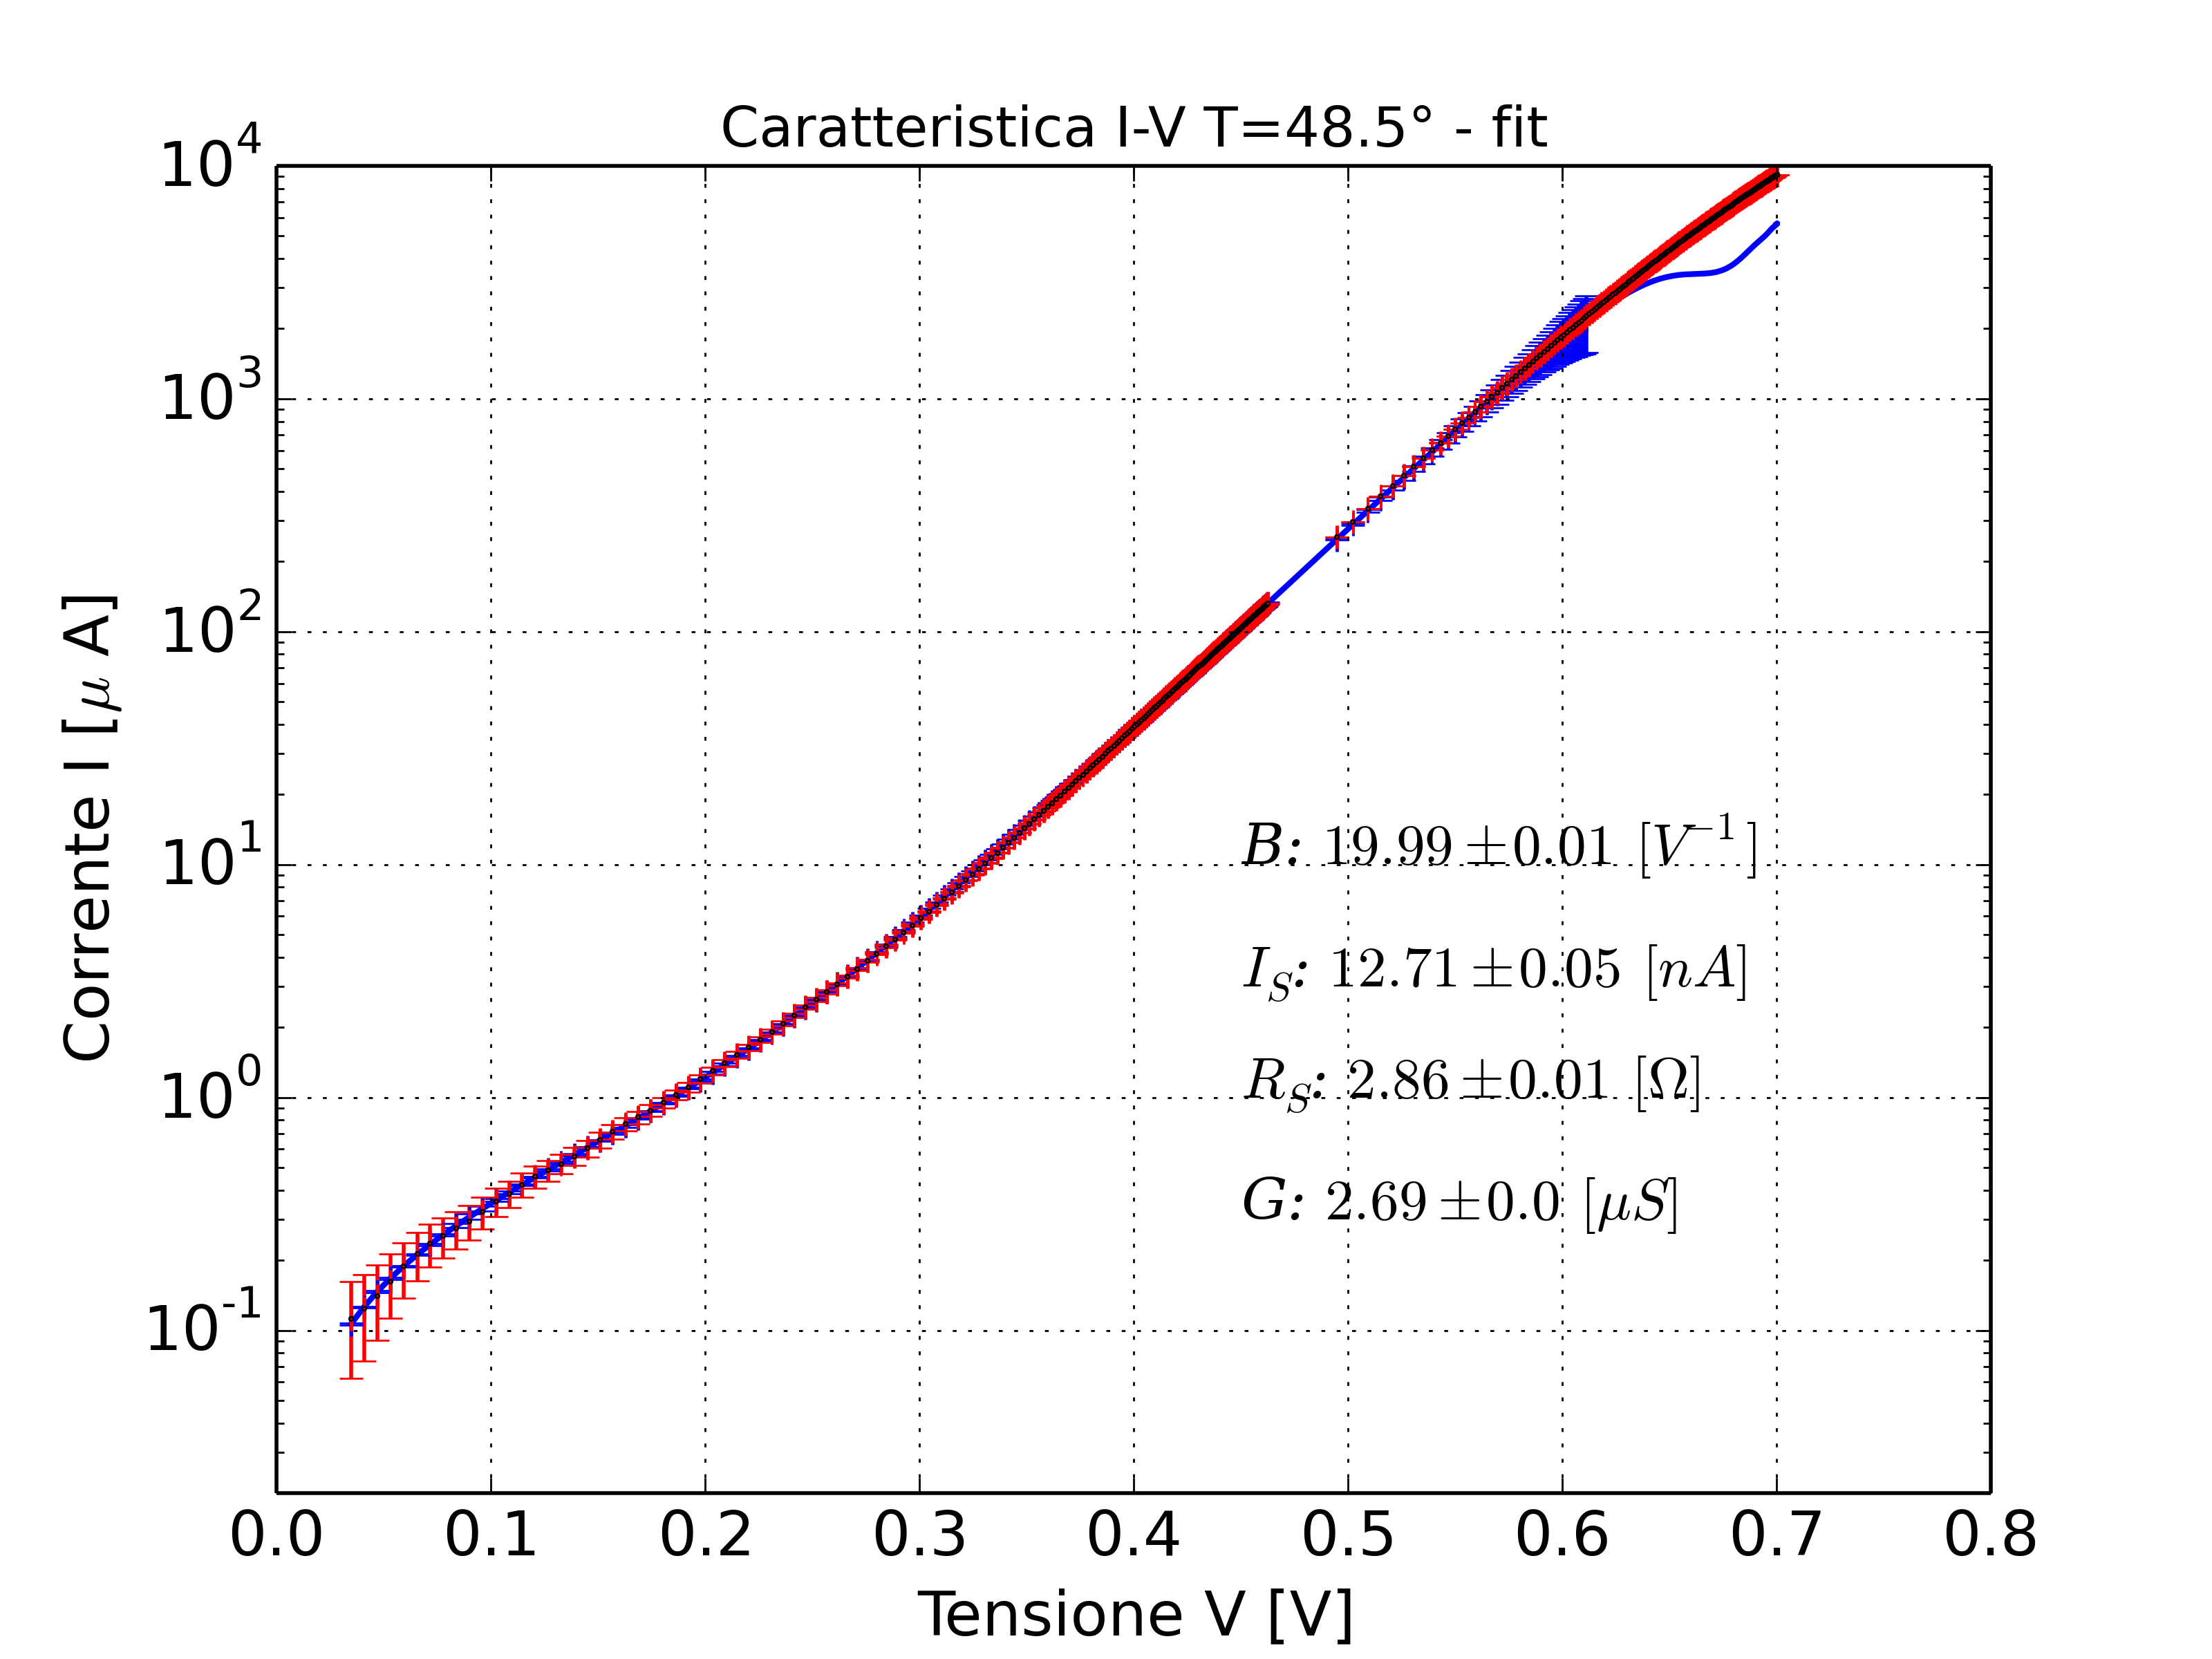
\includegraphics[width=0.5\linewidth]{./C9}}
\qquad
\subfloat[]{
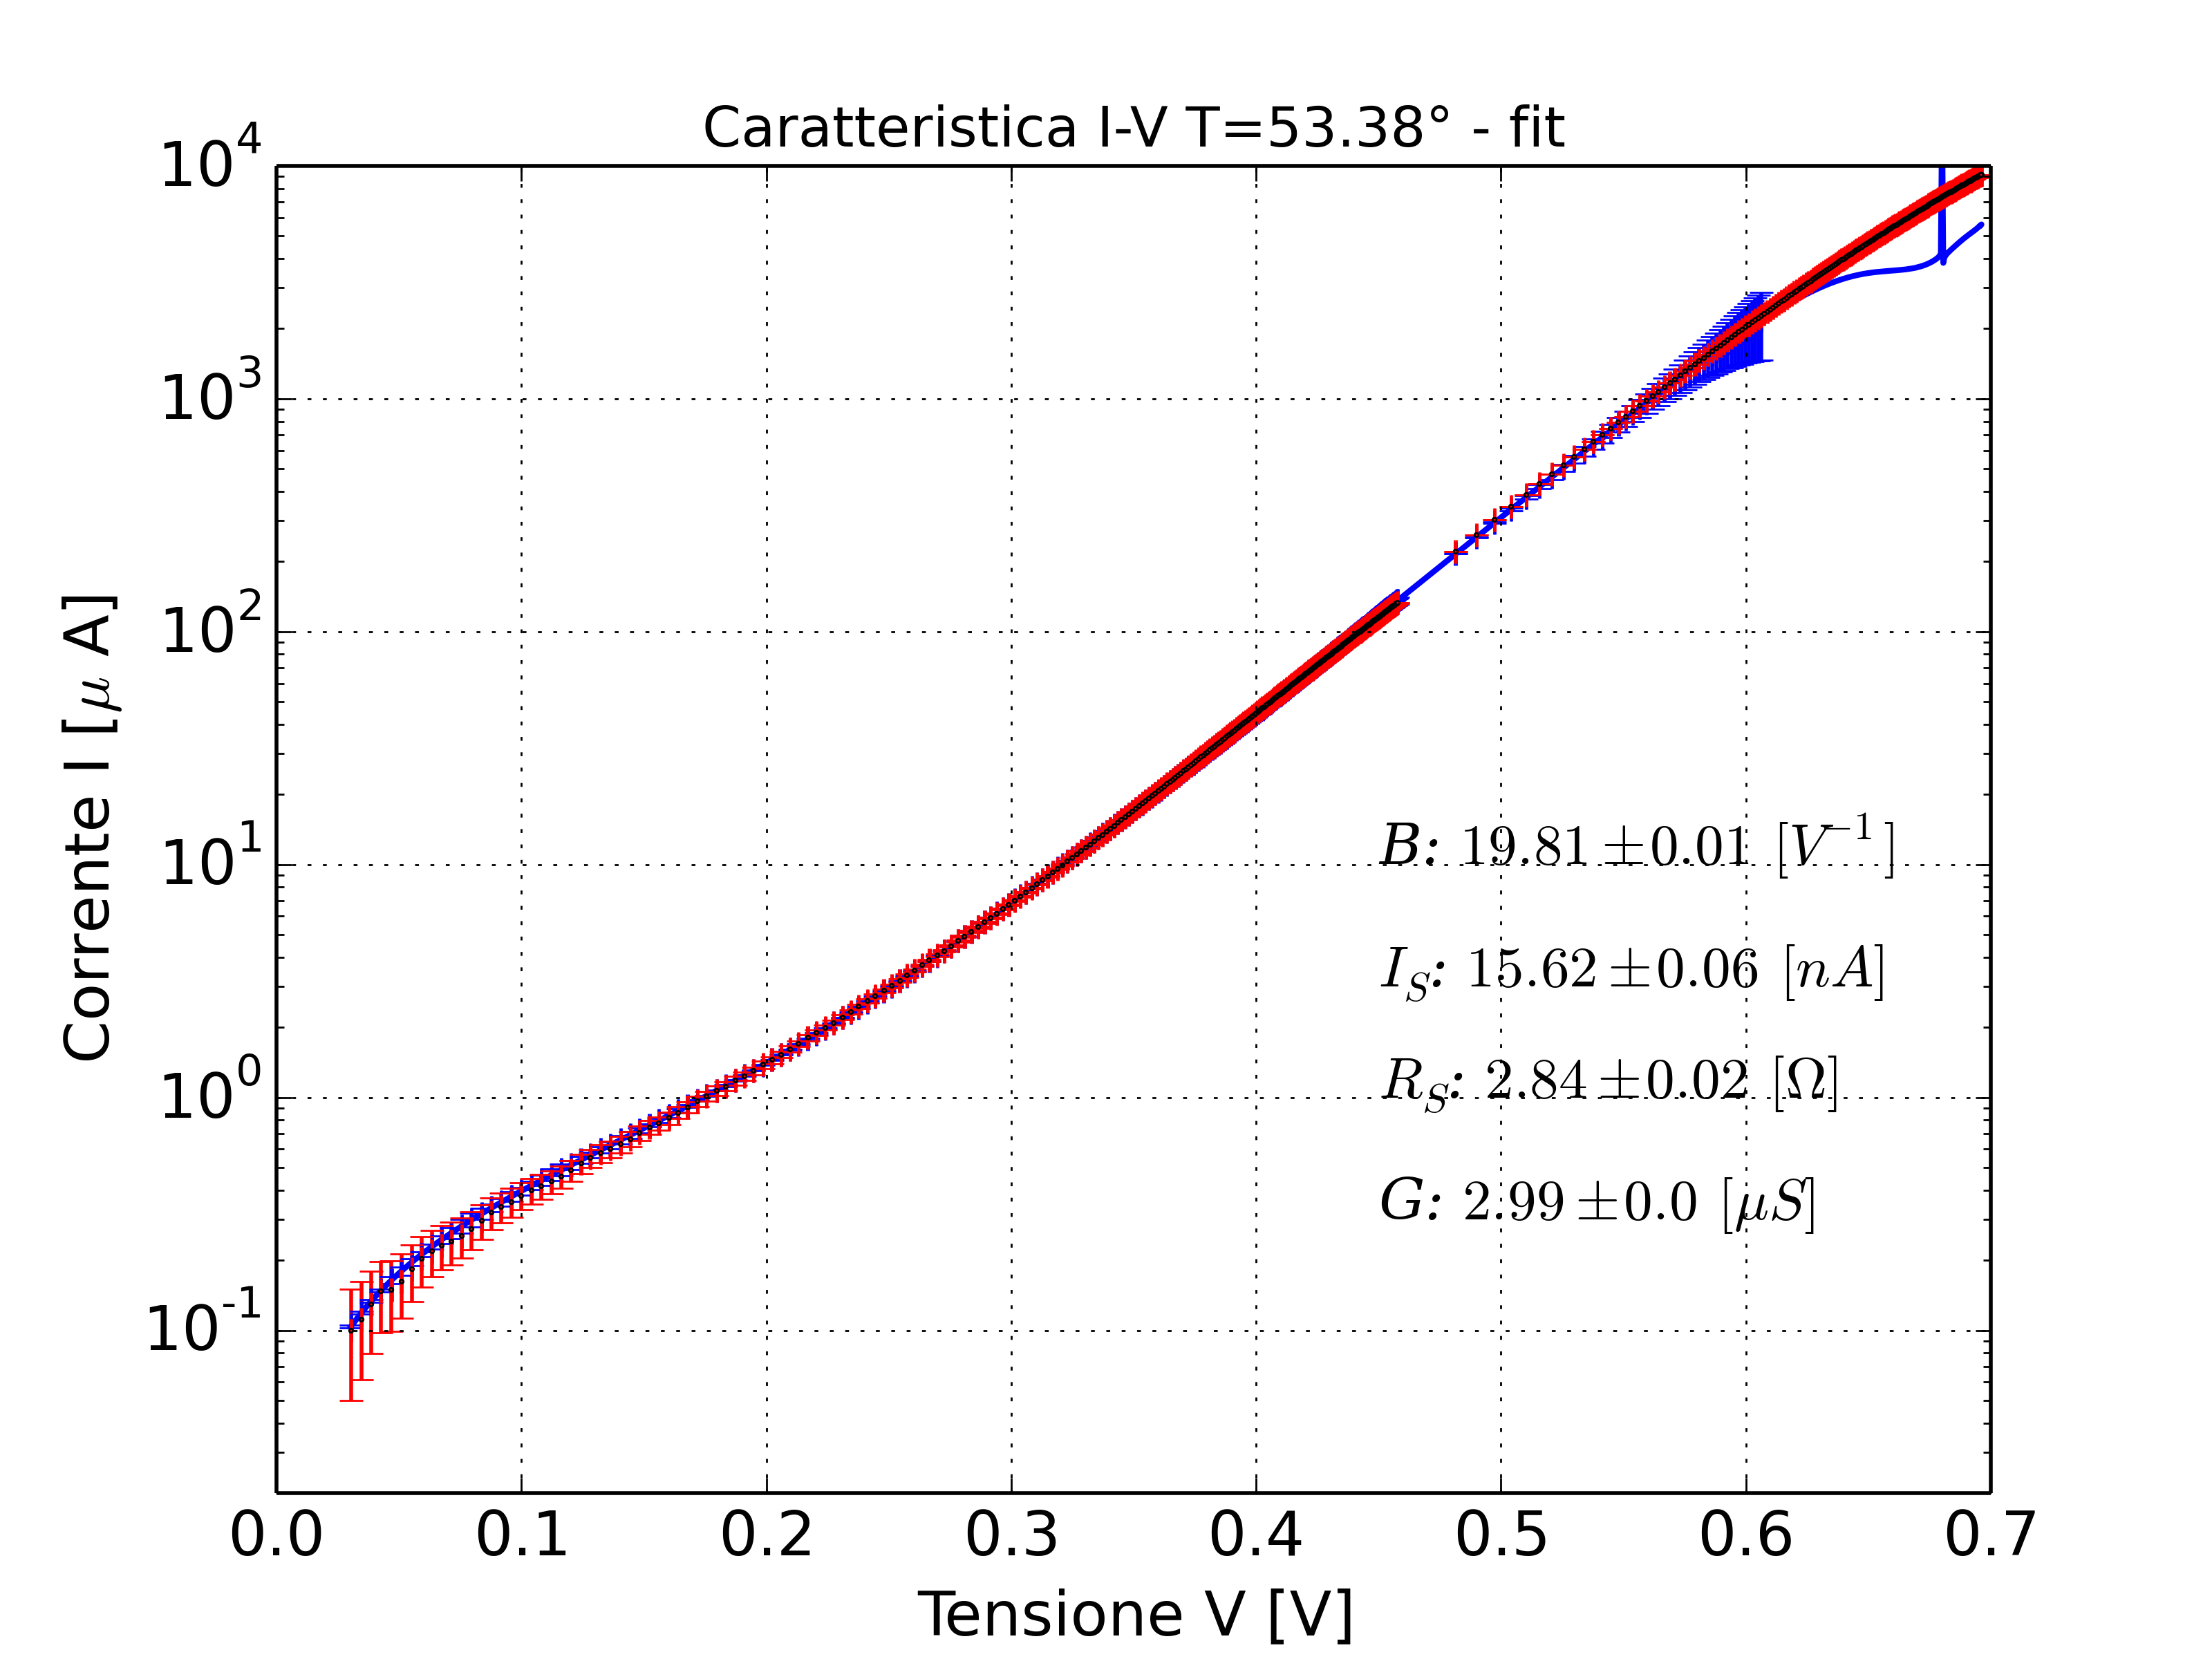
\includegraphics[width=0.5\linewidth]{./C10}}
\subfloat[]{
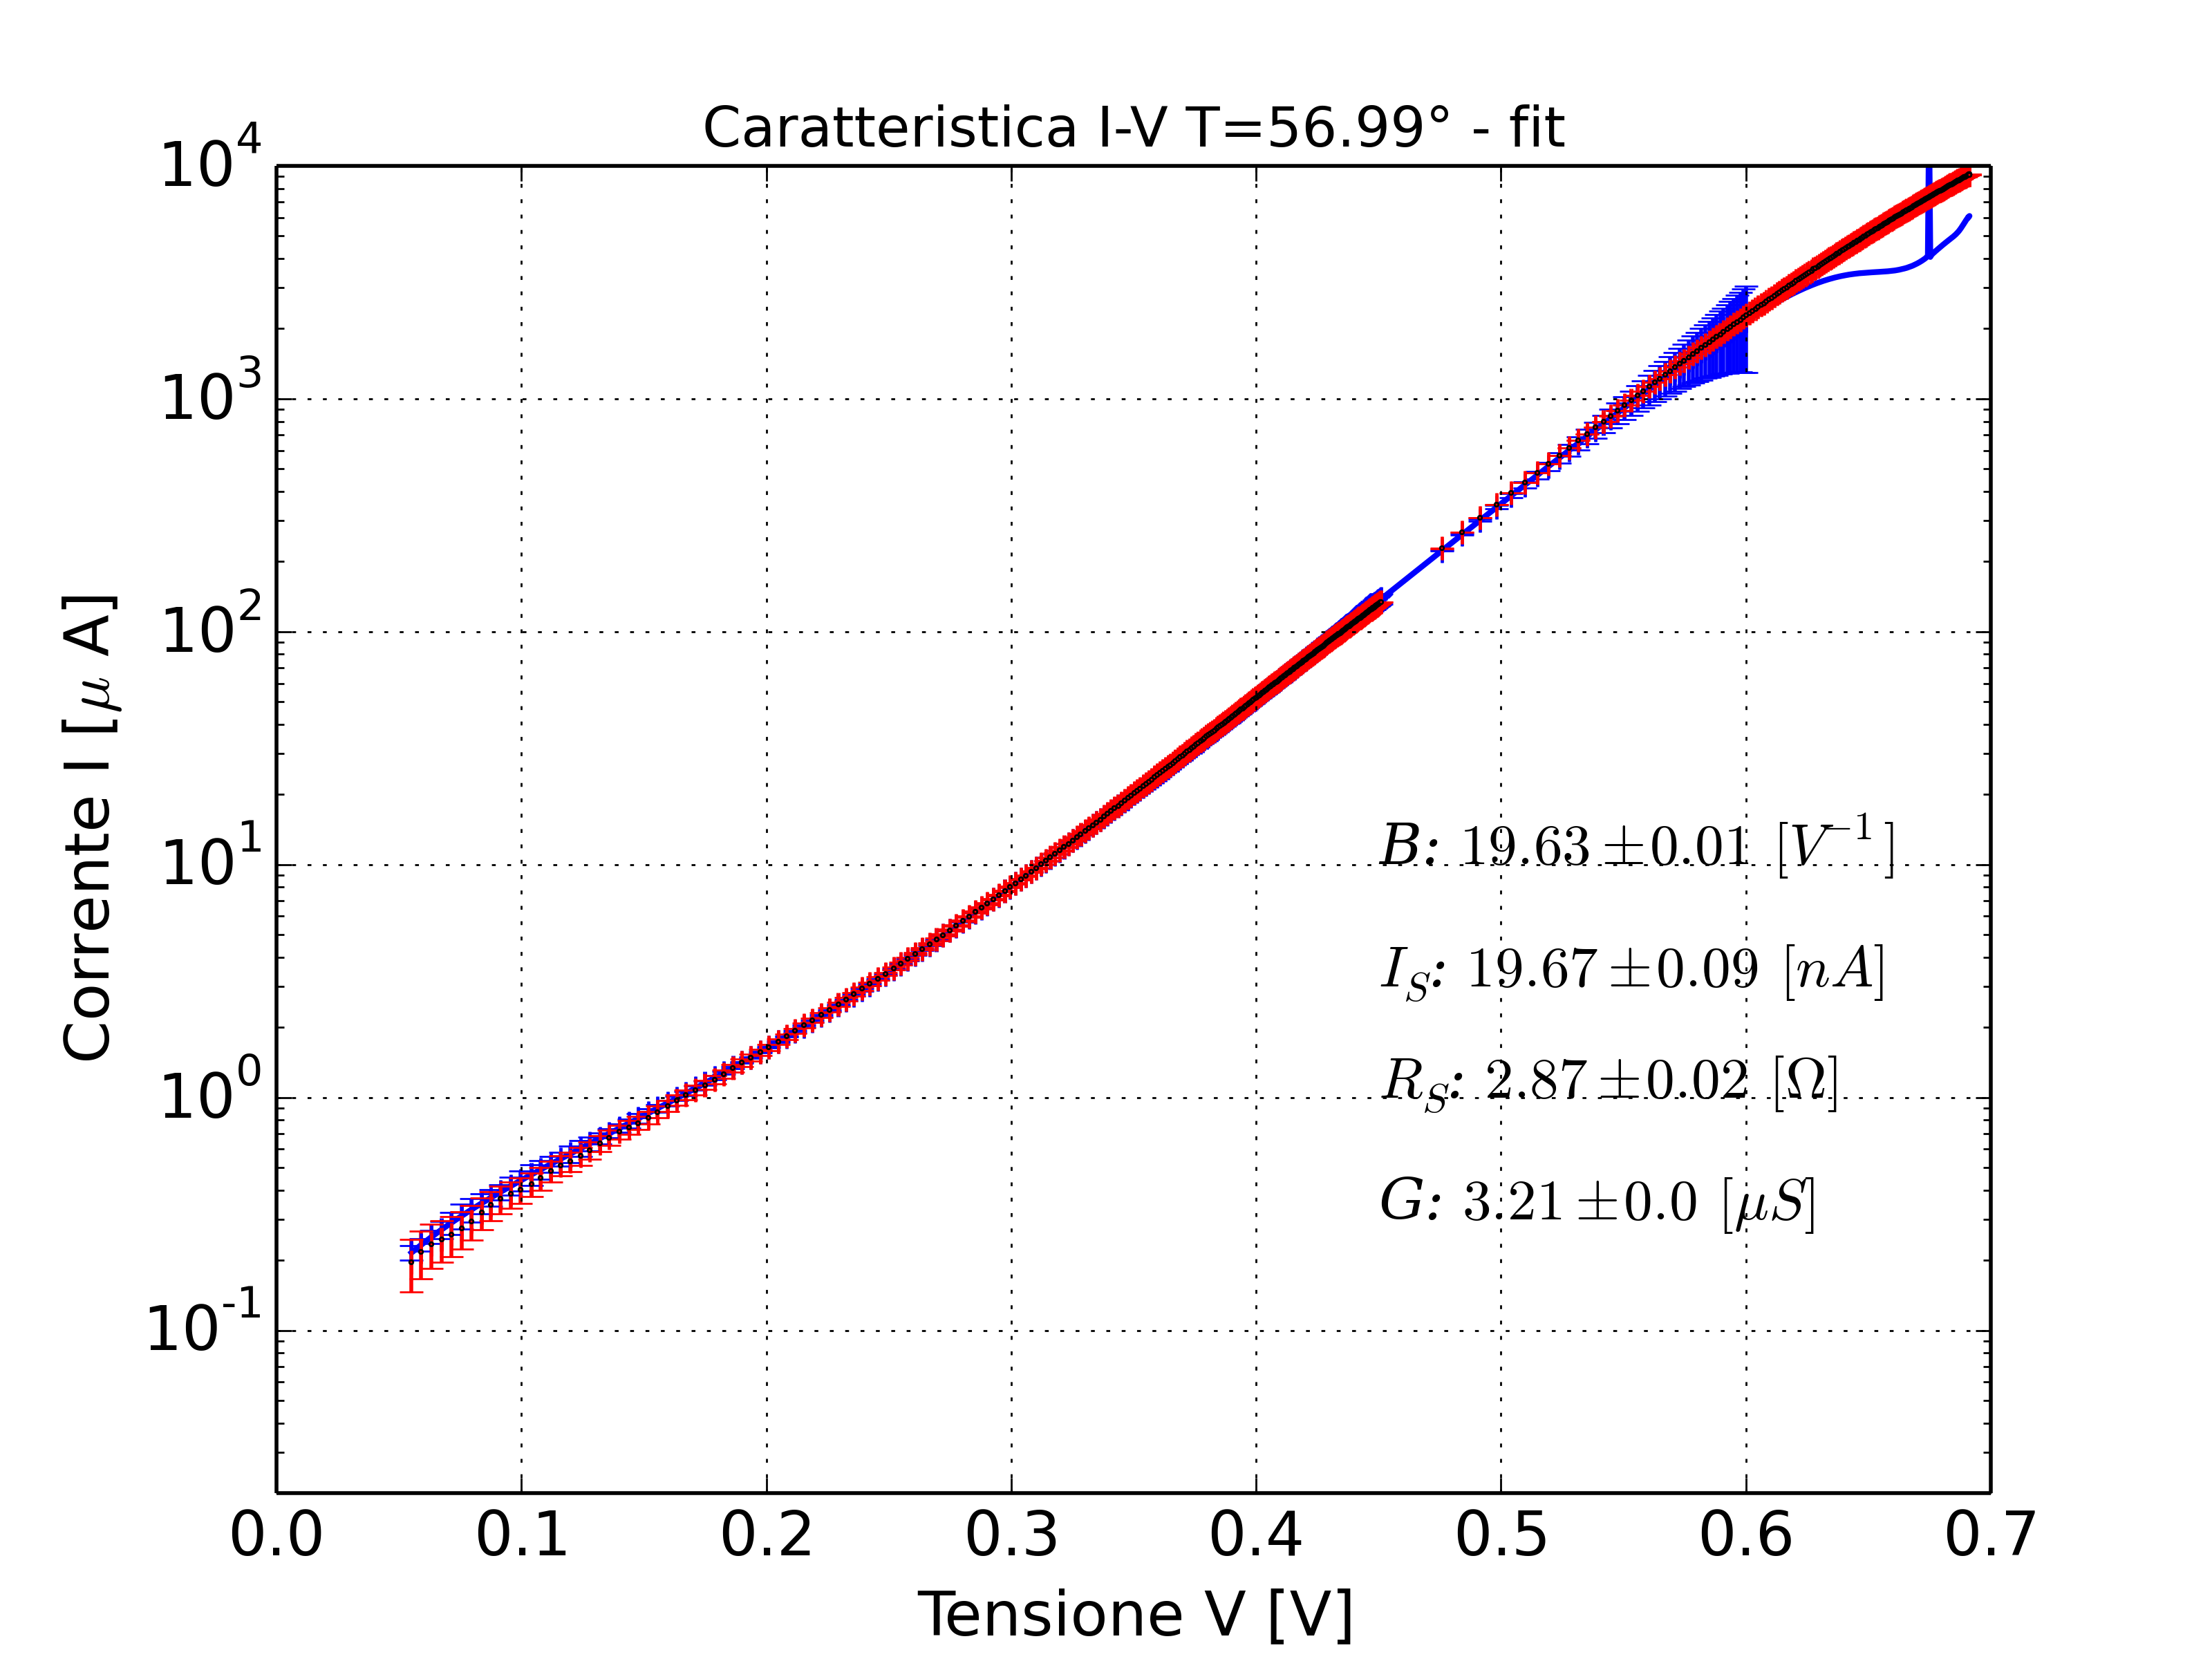
\includegraphics[width=0.5\linewidth]{./C11}}

\caption{Fit iterativo delle caratteristiche I-V per alcuni valori di T.}
\label{iterative_fit}
\end{figure}


Nella Tabella () di seguito si riassumono invece tutti i parametri dei fit ottenuti per le diverse temperature. Grazie al gran numero di misure a disposizione, è possibile evidenziare degli andamenti di questi parametri in funzione della temperatura, come è stato fatto in Figura (\ref{params}).

\begin{table}[h]
\centering
% This LaTeX table template is generated by emacs 24.3.1
\begin{tabular}{c|c|c|c|c|c|c|c|c}
\hline
\textbf{B} [$V^{-1}$]& $\delta$B & $\textbf{I}_s$ [nA]& $\delta I_S$ & $\textbf{R}_s$ $\Omega$ & $\delta$R & \textbf{G} [$\mu$S]& $\delta$G & Temp(errore0.5°C) \\
\hline
21.33 & 0.04 & 1.49 & 0.03 & 1.89 & 0.06 & 2.11 & 0.01 & 15.86 \\

21.31 & 0.03 & 1.69 & 0.03 & 1.93 & 0.05 & 2.16 & 0.03 & 18.63 \\

20.99 & 0.03 & 2.74 & 0.04 & 2.23 & 0.05 & 2.22 & 0.04 & 25.75 \\

20.75 & 0.02 & 3.84 & 0.04 & 2.37 & 0.04 & 2.28 & 0.03 & 30.94 \\

20.68 & 0.02 & 4.88 & 0.04 & 2.56 & 0.03 & 2.39 & 0.05 & 35.43 \\

20.448 & 0.011 & 6.26 & 0.04 & 2.57 & 0.03 & 2.43 & 0.07 & 38.78 \\

20.277 & 0.013 & 8.55 & 0.05 & 2.744 & 0.019 & 2.54 & 0.04 & 43.84 \\

20.284 & 0.012 & 8.76 & 0.03 & 2.763 & 0.015 & 2.6 & 0.04 & 44.64 \\

19.993 & 0.008 & 12.70 & 0.05 & 2.857 & 0.014 & 2.69 & 0.06 & 48.5 \\

19.812 & 0.008 & 15.62 & 0.06 & 2.844 & 0.015 & 2.99 & 0.08 & 53.38 \\

19.623 & 0.014 & 19.66 & 0.09 & 2.86 & 0.02 & 3.21 & 0.07 & 56.99 \\

19.582 & 0.011 & 21.72 & 0.11 & 2.92 & 0.02 & 3.40 & 0.07 & 58.92 \\

19.57 & 0.02 & 23.47 & 0.15 & 2.90 & 0.03 &   3.61 & 0.07 & 60.53 \\

19.54 & 0.02 & 25.058 & 0.19 & 2.92 & 0.03 &  3.81 & 0.08 & 62.06 \\

19.183 & 0.011 & 33.60 & 0.13 & 2.85 & 0.02 & 3.8 & 0.1 & 65.18 \\
\hline
\end{tabular}
\end{table}


\begin{itemize}
\item Nel caso della corrente di saturazione (\ref{fig:parametro_I}), l'andamento sembra essere grossomodo esponenziale, come ci si aspetta. \\
\item Il parametro B diminuisce all'aumentare della temperatura T (\ref{fig:parametro_B}): dalla definizione si ha $B = e/nkT$, per cui la relazione dovrebbe essere di tipo iperbolico; tuttavia, per la particolare regione esplorata dei valori di B, questo si può approssimare piuttosto bene con una relazione lineare, da cui il grafico.\\
\item Il parametro G (\ref{fig:parametro_G}), che rappresenta l'ammittanza della resistenza in parallelo al diodo, (è un reciproco di una resistenza), aumenta in maniera evidente con T, quindi la resistenza in parallelo diminuisce: sembra quindi che per alte T, nel regime di basse correnti dove il parametro G ha un incidenza maggiore (si rimanda alla discussione sulle deviazioni dal modello di Schockley), la corrente che scorre in questa resistenza parallela diventi sempre meno trascurabile.\\
\item Infine, la resistenza in serie $R_S$ tende ad aumentare con T (\ref{fig:parametro_R}), e questo è compatibile con la nota relazione fra resistività di un conduttore e temperatura, nonostante ad un certo punto sembri diventare stazionaria o addirittura diminuire (non ci sono abbastanza dati in quella regione per stabilirlo). Si tenga presente, comunque, che la descrizione lineare dell'aumentare della resistività in funzione della temperatura è un'approssimazione valida solo per range limitati, al di fuori dei quali non rappresenta più un modello esaustivo.
\end{itemize}

\begin{figure}
\centering
\subfloat[Subfigure 1 list of figures text][Andamento di B in funzione della temperatura T]{
\includegraphics[width=0.5\linewidth]{./parametro_b_temp}
\label{fig:parametro_B}}
%\qquad
\subfloat[Subfigure 2 list of figures text][Andamento di G in funzione di T.]{
\includegraphics[width=0.5\linewidth]{./parametro_g_temp}
\label{fig:parametro_G}}
\qquad
\subfloat[Subfigure 1 list of figures text][Andamento della corrente di saturazione $I_S$ in funzione di T.]{
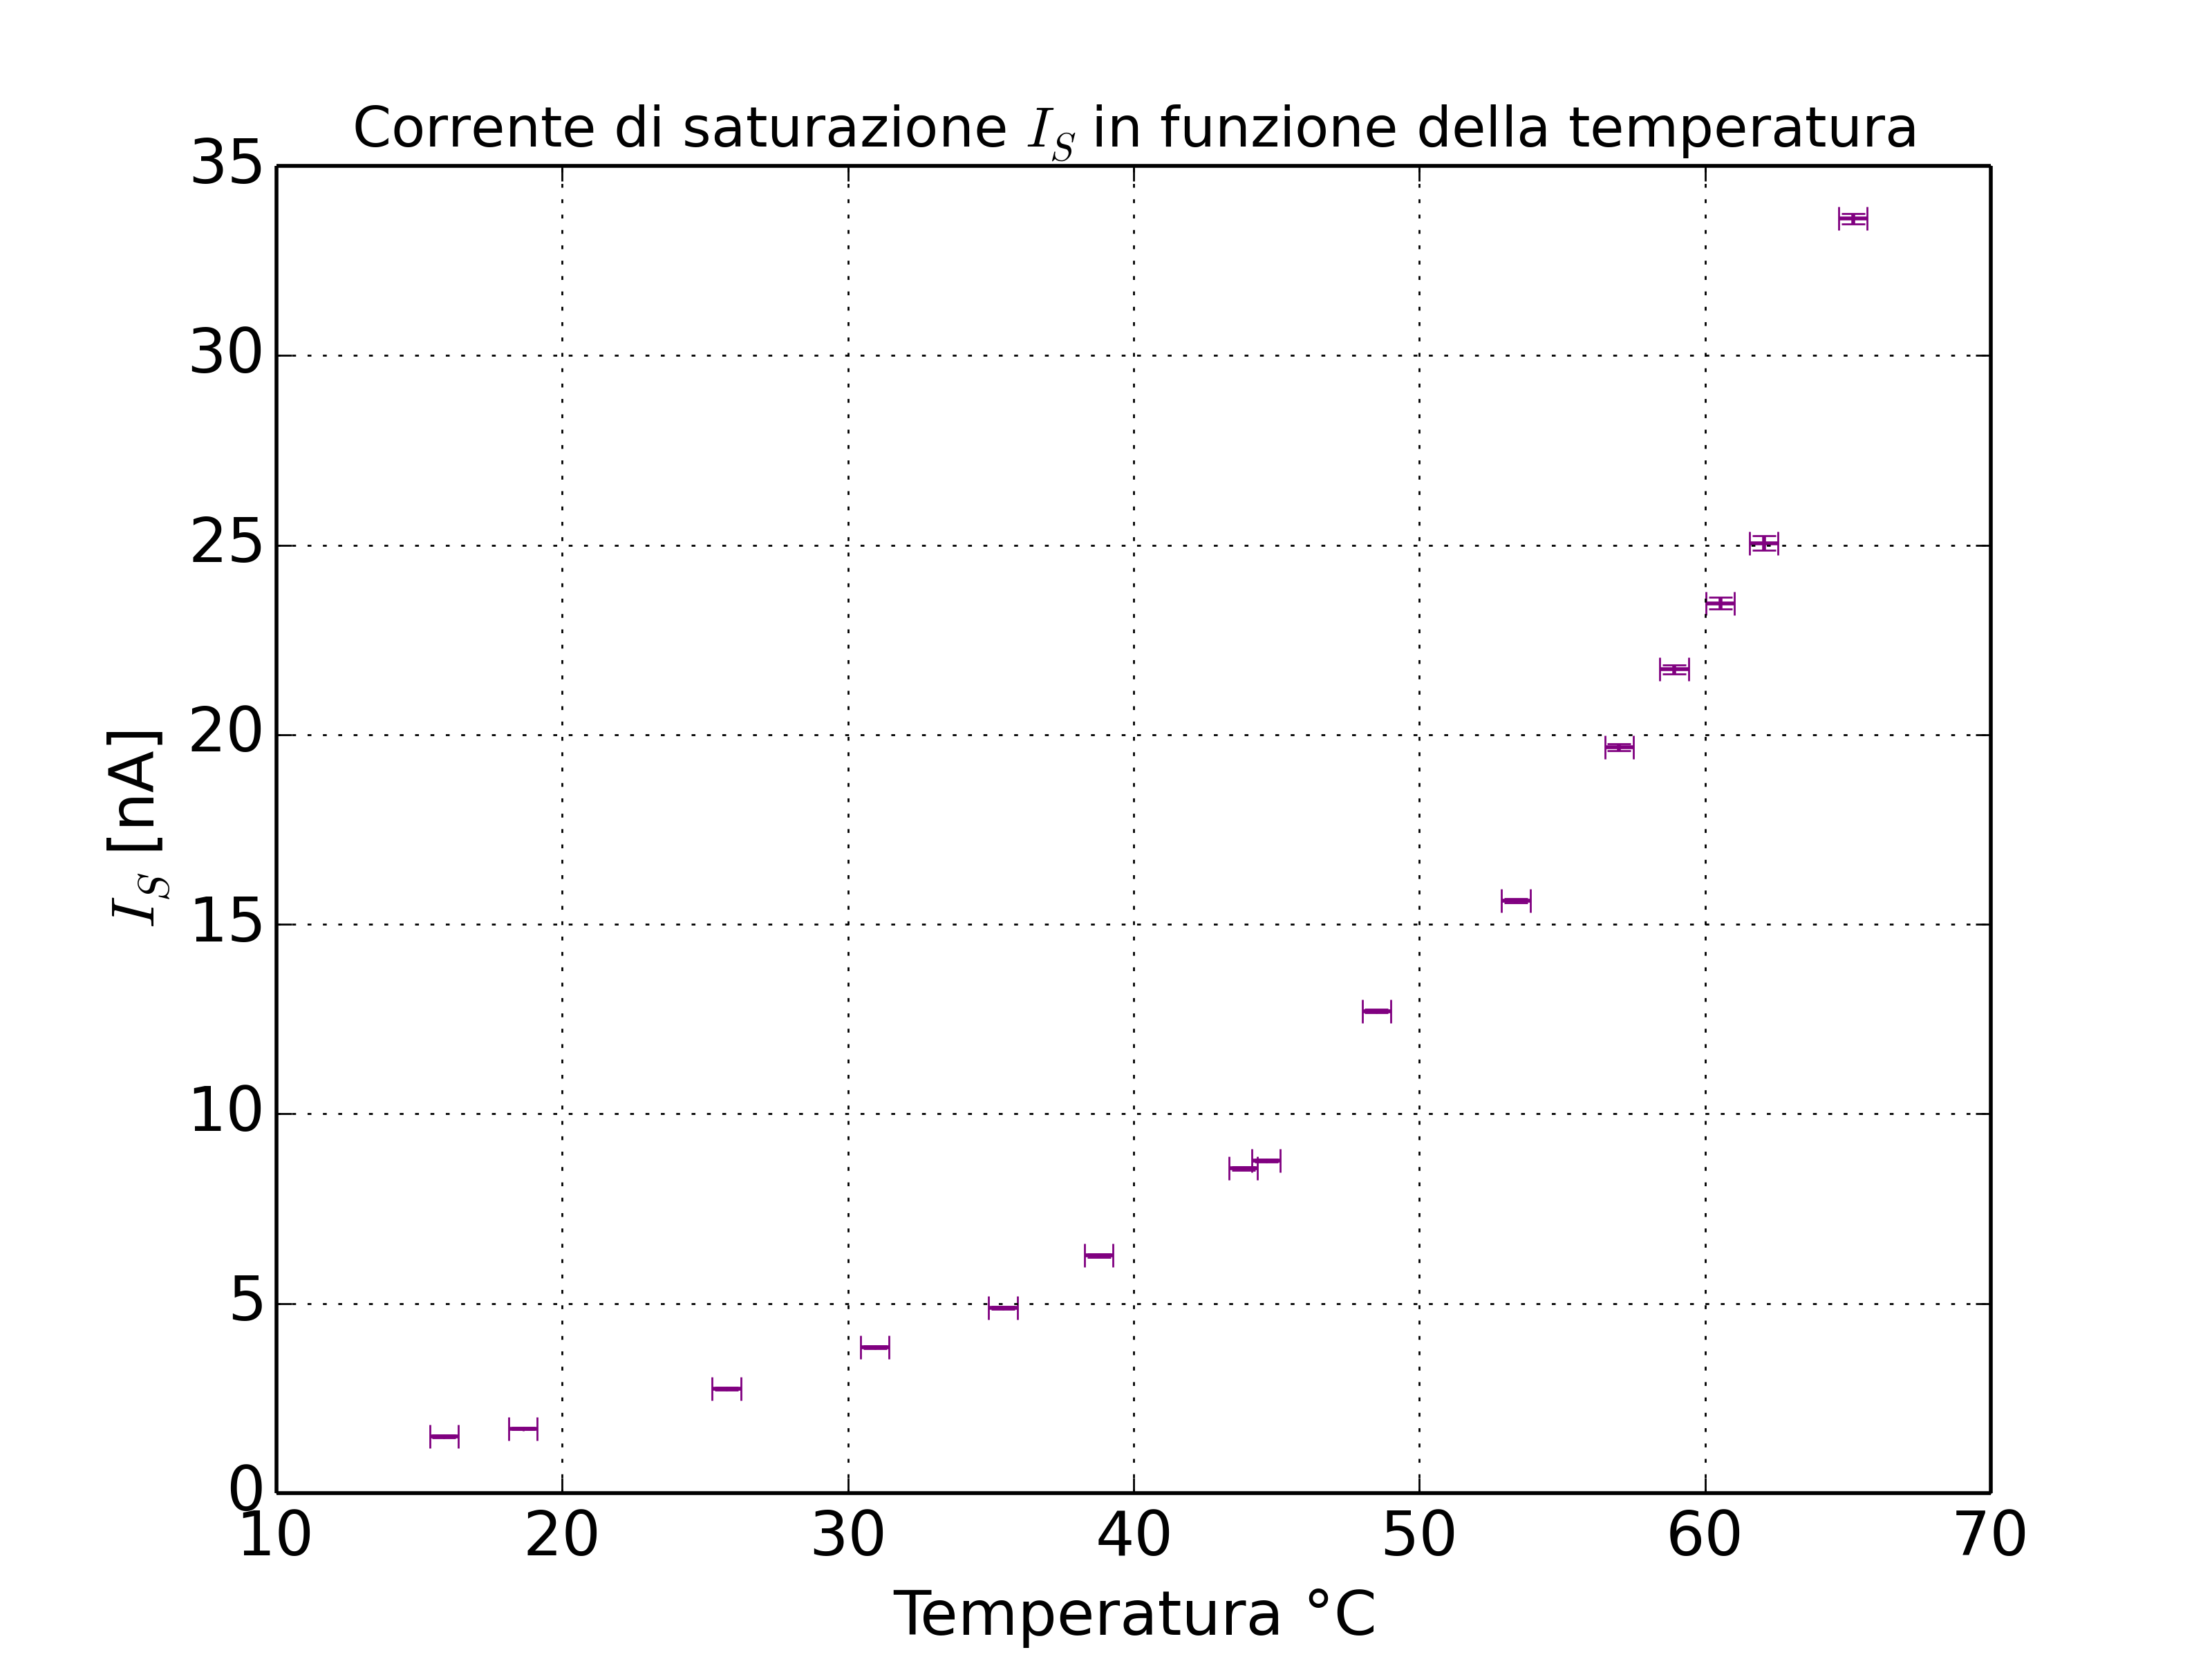
\includegraphics[width=0.5\linewidth]{./parametro_Is_temp}
\label{fig:parametro_I}}
%\qquad
\subfloat[Subfigure 2 list of figures text][Andamento della resistenza in serie $R_S$ in funzione di T.]{
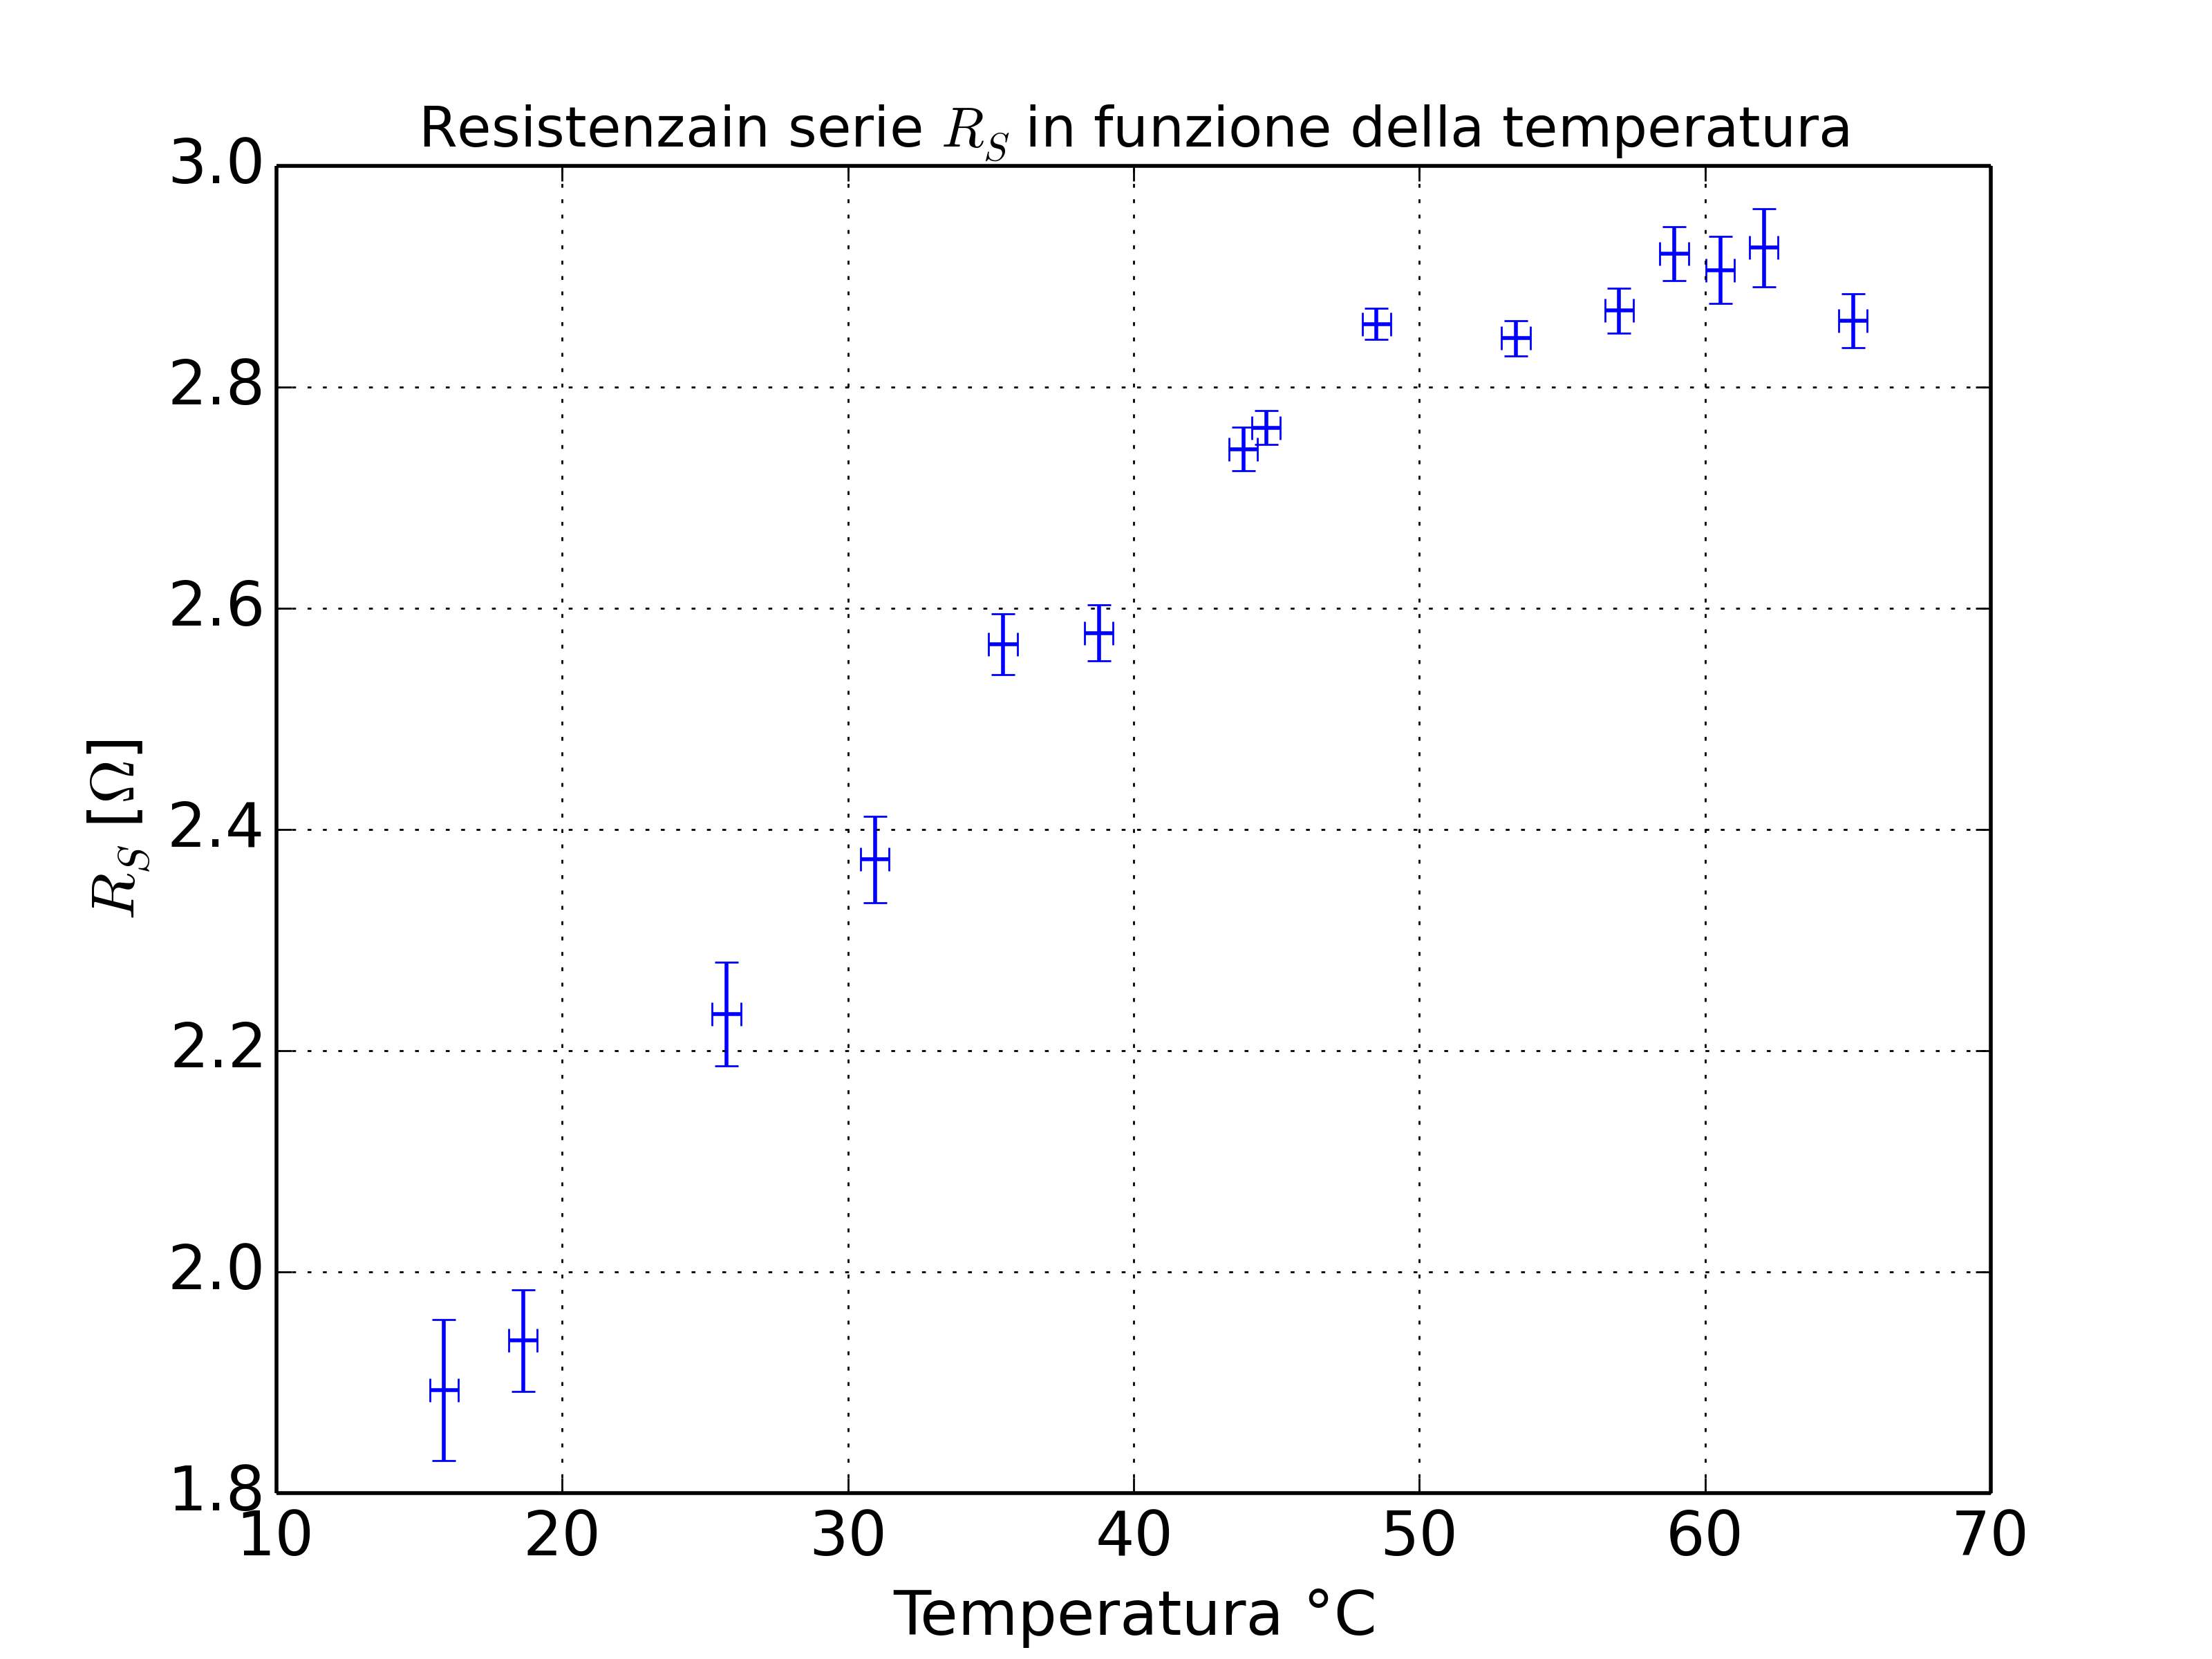
\includegraphics[width=0.5\linewidth]{./parametro_Rs_temp}
\label{fig:parametro_R}}
\caption{Parametri del fit: andamento in T.}
\label{params}
\end{figure}

\begin{thebibliography}{10}
\bibitem{bib1}
Lorem M, Ipsum VE (1990) Rank Correlation Methods. New York: Oxford University Press, 5th edition.

\bibitem{bib2}
Ipsum M, Ipsum JD (1990) Rank Correlation Methods. New York: Oxford University Press, 5th edition.

\end{thebibliography}



\end{document}